\documentclass{article}
\usepackage[utf8]{inputenc}
\usepackage[english]{babel}
\usepackage{titlesec}
\usepackage{hanging}
\usepackage{indentfirst}
\usepackage{setspace}
\usepackage{float}
\usepackage{multirow}
\usepackage{mathrsfs}
\usepackage{caption}
\usepackage{tocbasic}
\usepackage[toc,page]{appendix}
\usepackage[table,xcdraw]{xcolor}
\usepackage{longtable}
\usepackage{listings}
\usepackage{amsmath}
\DeclareTOCStyleEntry[beforeskip=.1em plus 1pt, pagenumberformat=\textbf]{tocline}{section}
\usepackage{adjustbox}
\usepackage[english]{babel}
\setlength{\parindent}{4em}
\setlength{\parskip}{0.5em}
\usepackage{array}
\usepackage{hyperref}
\hypersetup{
    colorlinks=false,
    linkcolor=black,
    filecolor=black,
    urlcolor=black,
}
\newcommand{\MYhref}[3][blue]{\href{#2}{\color{#1}{#3}}}%
\urlstyle{same}
\usepackage[letterpaper, portrait, margin=1in]{geometry}
\usepackage{graphicx}
\graphicspath{ {images/} }
\usepackage{array}
\newcolumntype{L}[1]{>{\raggedright\let\newline\\\arraybackslash\hspace{0pt}}m{#1}}
\newcolumntype{C}[1]{>{\centering\let\newline\\\arraybackslash\hspace{0pt}}m{#1}}
\newcolumntype{R}[1]{>{\raggedleft\let\newline\\\arraybackslash\hspace{0pt}}m{#1}}

\titleclass{\subsubsubsection}{straight}[\subsection]

\newcounter{subsubsubsection}[subsubsection]
\renewcommand\thesubsubsubsection{\thesubsubsection.\arabic{subsubsubsection}}

\titleformat{\subsubsubsection}
  {\normalfont\normalsize\bfseries}{\thesubsubsubsection}{1em}{}
\titlespacing*{\subsubsubsection}
{0pt}{3.25ex plus 1ex minus .2ex}{1.5ex plus .2ex}

\makeatletter
\renewcommand\paragraph{\@startsection{paragraph}{5}{\z@}%
  {3.25ex \@plus1ex \@minus.2ex}%
  {-1em}%
  {\normalfont\normalsize\bfseries}}
\renewcommand\subparagraph{\@startsection{subparagraph}{6}{\parindent}%
  {3.25ex \@plus1ex \@minus .2ex}%
  {-1em}%
  {\normalfont\normalsize\bfseries}}
\def\toclevel@subsubsubsection{4}
\def\toclevel@paragraph{5}
\def\toclevel@paragraph{6}
\def\l@subsubsubsection{\@dottedtocline{4}{7em}{4em}}
\def\l@paragraph{\@dottedtocline{5}{10em}{5em}}
\def\l@subparagraph{\@dottedtocline{6}{14em}{6em}}
\makeatother

\setcounter{secnumdepth}{4}
\setcounter{tocdepth}{4}

\renewcommand{\contentsname}{Table of Contents}
\renewcommand{\listtablename}{Tables}
\renewcommand{\listfigurename}{Figures}





%========================%
% Beginning of Document  %
%========================%

\begin{document} 





%========================%
%       Title Page       %
%========================%

\pagenumbering{gobble}
\begin{center}
    \Huge{\textbf{Evaluation of reliability of a technical system}}
    \\ 
    \vspace{10mm}
    \large{
    Final project for the course of \\
    Articial Neutral Networks 214350 \\
    part of the faculty of\\
    Electrical Engineering and Informatics\\
    from the \\
    Zittau/Görlitz University of Applied Sciences\\
    }
    \Large{
    \vspace{15mm}
    {\huge B. Eng. Automation and Mechatronics} \\
    \vspace{15mm} 
    {\LARGE By:} \\
    \vspace{5mm}
    Jesús Jair Reyes Gutiérrez \\
    \vspace {15mm}
    {\LARGE Project Advisor:} \\
    \vspace{5mm}
    Prof. Dr.-Ing. W. Kästner \\
    \vspace {15mm}
    {\LARGE Project level:}\\ 
    \vspace{5mm}
    Bachelor\\ 
    \vspace {15mm}
    Date: January 2021 \\ 
    }
    \vspace{15mm}
    \large{\textit{This report represents the work of an undergraduate student for a class part of his DHIK double degree program between the Mexican university "Instituto Tecnológico y de Estudios Superiores de Monterrey" and the German Hochschule "Hochschule Zittau/Görlitz".}}
\end{center}





%========================%
%        Abstract        %
%========================%

\newpage
\pagenumbering{roman}
\setcounter{page}{1}

\section*{Abstract}

\par Throughout the pages of this paper, the process followed to design and develop a Hybrid Markov Model by training a multilayer perceptron with a pre-established data set will be presented, explained and detailed. DataEngine software was used for the realization of the multilayer perceptron, Excel and MatLab were used for the preparation and pre-processing of the data, and Dynstar was used for the implementation of the hybrid Markov model using a Soft Computing model.

\par Additionally, a brief theoretical framework will be presented with all the necessary concepts to understand each part of the process, as well as the results of each stage, to finally compare the results of the hybrid model with the classical one. At each stage, the justifications for each decision will be included, along with its corresponding implementation. 





%========================%
%     Acknowledgements   %
%========================%

\newpage
\section*{Acknowledgements} 

\par I have to start by thanking my professor of Artificial Neutral Networks, Prof. Dr.-Ing. W. Kästner. For providing me with the necessary knowledge to understand what a Markov model is and thus subsequently to understand each step of the design process. Additionally, I also thank him for his mentoring during the development of the whole project.





%========================%
%    Table of Contents   %
%========================%

\newpage 
\tableofcontents
\listoftables
\listoffigures





%========================%
%       Introduction     %
%========================%

\newpage 
\begin{doublespacing}
\pagenumbering{arabic}
\setcounter{page}{1}

\section{Introduction}

\par Over time, the tools, machinery and systems of industry have facilitated mass production, thanks in large part to technological advances that have made them more complex, efficient and durable. However, this progress has also posed a great challenge for engineers and operators, since their complexity prevents the development of models that are 100\% adjusted to reality and forces them to be simplified. Therefore, the development of reliable models is one of the greatest challenges of modern industry, since with them it is not only possible to determine the scope of current equipment or processes, but it is also possible to make very accurate forecasts. One of the most relevant forecasts is the one that determines how often it is necessary to perform maintenance on a tool, machinery or system, because maintenance involves not only expenses in itself, but also in production due to downtime. 

\subsection{Project Aim}

\par For this reason, this paper proposes to evaluate the reliability of a model based on a hybrid Markov model against that of a classical model.  For this purpose, a set of data will be presented that will go through different stages to create a multilayer perceptron, which will be subsequently implemented in a computational Markov model, which, based on a stress scenario of temperature and humidity, will provide a forecast of the time required to provide maintenance to the process or system under analysis.

\par The following is a brief explanation of each of the stages through which the initial data set will pass until the objective is met. 

\subsubsection{Data pre-processing}

\par Through this first stage, the first filter of the information received will be carried out, because although it is information received directly from the source, the measurements may contain errors that must be eliminated for the subsequent stages

\subsubsection{Data preparation} 

\par In this second filtering stage, the data must be separated for the training and testing of the multilayer perceptron, but, in order to guarantee efficiency, it is necessary to distribute the data in an intelligent way.

\subsubsection{MLP design} 

\par This third stage consists directly in designing a multilayer perceptron in the selected software, under certain parameters that guarantee the maximum and minimum error requirements established, in this case, of $ \pm 3\%$. 

\subsubsection{Mathematical models} 

\par This stage presents the design of the Markov model under ideal conditions, which will lead to the calculation of the expected or desired results.

\subsubsection{Simulation models} 

\par The Markov model will be implemented in a simulation software. For this purpose, the classical and hybrid models will be included in order to generate a comparison. 

\subsubsection{Simulation results} 

\par At this stage, the results obtained in both models, the classical and the hybrid, will be presented,and it is going to be described their empirical properties, without any further or really deep analysis.

\subsubsection{Evaluation} 

\par Finally, the results obtained will be evaluated, compared, analyzed and interpreted to issue a conclusion about the time required to maintain the analyzed process or equipment. Here the two models, classical, and hybrid will be compared.

\subsection{Background} 

\par It is worth mentioning that this project is the result of the Articial Neutral Networks 214350 class given by Prof. Dr.-Ing. W. Kästner. Through this class all the necessary knowledge for the realization of this project was provided, as well as all the technological tools for its development. As already mentioned, DataEngine, MatLab, Excel and Dynstar were the software used in the development of the project. 





%========================%
%          Theory        %
%========================%

\newpage 
\section{Theory and Methodology}

\par First of all, we must begin by defining the importance and necessity of modelling and simulating physical phenomena. Thanks to these tools, it is possible to make prognoses about reality and generate knowledge about the causes that led to the result obtained, as well as what would have happened if something different had been done \cite{kaestner:basics}. Furthermore, modelling and simulating the behavior of a system is not only restricted to a single area, but its application framework ranges from engineering to medicine and social sciences \cite{kaestner:basics}.

\par With this in mind, in order to model any system, it is first necessary to take into account how much is known about it, as well as its characteristics. 
 

\subsection{System} 
{
\par A system is a set of components that interact with each other and it is thanks to these interactions that a system is more than just the sum of its components \cite{kaestner:basics}. In addition, a system must have a purpose that, together with the structure of its components, gives it an identity \cite{kaestner:basics}. And finally, some other characteristics or parts of systems are their inputs and outputs, both coming from or going out of the system boundaries \cite{kaestner:basics}. The inputs being totally independent and the outputs depending totally on the system process, which is characterized by its internal or state variables \cite{kaestner:basics}. 

\begin{figure}[H] 
    \centering
    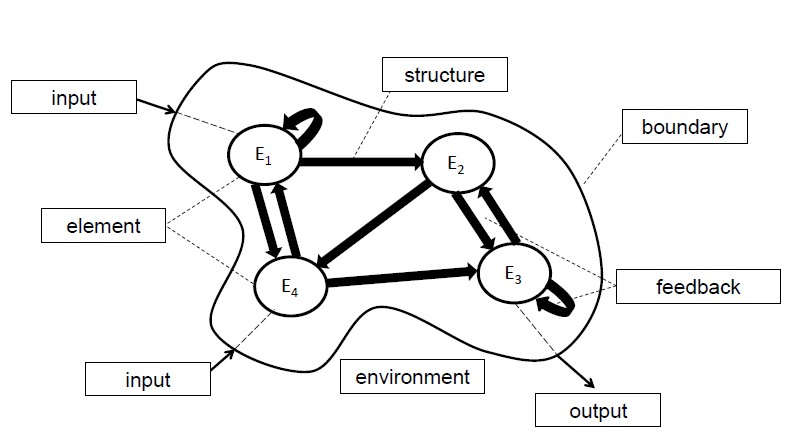
\includegraphics[width=0.8\textwidth]{Images/Partes_del_sistema.JPG} 
    \caption{System representation \cite{kaestner:basics}} 
    \label{fig:SystemParts} 
\end{figure}

\par As can be seen in Figure \ref{fig:SystemParts}, the system is contained by a boundary, in which the inputs enter, these pass between the elements of the system according to its structure, which can have feedback or changes in the system by the same change of the state variables \cite{kaestner:basics}. In general, a system works by causes and effects, an input arrives and depending on the organization and parameters of the system this is transformed into a desired output \cite{kaestner:basics}. 
}


\subsection{Model} 
{
\par On the other hand, a model is a simplified scale reproduction of some phenomenon \cite{kaestner:basics}. Models can be mathematical, conceptual or physical, although these will always be limited by the simplification, neglect, abstraction and aggregation they have made of reality \cite{kaestner:basics}. However, some minimum and indispensable requirements they must meet are verifiability and reproducibility in different environments \cite{kaestner:basics}. That is why, in order to favor the verifiability and reproducibility of the models, models can be described or classified in different ways:

\subsubsection{Linear or non-linear:}
\par If the input variable undergoes a proportional change with respect to the output, the superposition principle is satisfied and the steady state does not depend on the initial conditions \cite{kaestner:basics}.

\subsubsection{Static or dynamic:}
\par If the system does not change its behavior during the observation time \cite{kaestner:basics}.

\subsubsection{Externally influenced or autonomous:}
\par If the system is influenced by external variables, call it inputs \cite{kaestner:basics}.

\subsubsection{Location dependent or independent:}
\par If the state variables and parameters are interpreted as set, were their position in the system matter\cite{kaestner:basics}. 

\subsubsection{Deterministic or stochastic:}
\par If random external influences on the model are excluded \cite{kaestner:basics}.

\subsubsection{Time-invariant or time-variant:}
\par If the same behavior can be observed with the same initial conditions \cite{kaestner:basics}.

\subsubsection{Time continuous or discrete:}
\par If the state of the system is defined at all points in time \cite{kaestner:basics}.

\vspace{5mm}

\par Now that one has a better understanding of systems and models, an important step to consider before modeling is to decide whether the model will be a model of behavior or a system model. Depending on the decision, one will face different challenges that will require certain knowledge about the system itself.

\subsubsection{Model of behavior}
\par It is a reproduction of the general relationship between input and output without really knowing the internal mechanisms that lead to that change, as in a black box model.

\begin{figure}[H] 
    \centering
    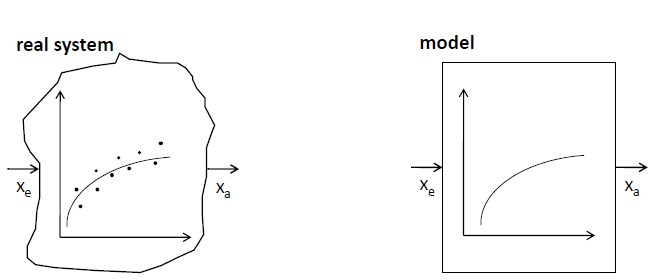
\includegraphics[width=0.8\textwidth]{Images/ModelOfBehavior.JPG} 
    \caption{Real system vs. Model of behavior \cite{kaestner:basics}} 
    \label{fig:ModelOfBehavior} 
\end{figure}

\par As can be seen in the Figure \ref{fig:ModelOfBehavior}, the model only tries to emulate the relationship between the input and output, so it is limited to the variations that may occur \cite{kaestner:basics}. To develop the model it is necessary to have a sufficiently large database of the input and output to ensure consistency and reproducibility \cite{kaestner:basics}.


\subsubsection{System model}
\par It is a reproduction of all the essential internal interactions of the system, so a deep knowledge of the system is required.

\begin{figure}[H] 
    \centering
    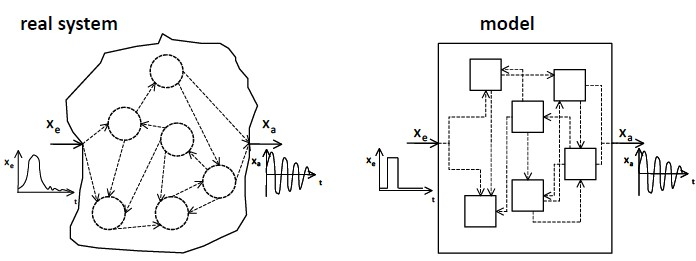
\includegraphics[width=0.8\textwidth]{Images/SystemModel.JPG} 
    \caption{Real system vs. System model \cite{kaestner:basics}} 
    \label{fig:SystemModel} 
\end{figure}

\par As can be seen in the Figure \ref{fig:SystemModel}, the most essential internal interactions have to be reproduced in order to approximate the behavior as closely as possible, so the model is limited to the accuracy of the reproduction of the system \cite{kaestner:basics}. The system model is most recommended for systems in which there are many non-linearities, the structure is very complex or unknown conditions are to be analyzed \cite{kaestner:basics}.
}

\subsection{Simulation} 
\par For the next step, simulation, it is first necessary to design the model, defining the system from its purpose, structure, boundaries and interactions. Then choose the type of model, quantify it, program it and verify it. Then choose the software, implement it, analyze it and validate it. To finally analyze the behavior and look for possible optimizations. It should be clarified that errors can come from different sources, such as the model itself, data linearization, model discretization, iterations, programming or rounding \cite{kaestner:basics}.

\subsection{Soft Computing}
\par In the case of behavioral modeling, it is necessary to integrate certain data analysis techniques to correctly model the behavior of the system. Some of the most common techniques are artificial neural network and fuzzy set theory, as they allow the modeling of nonlinear multivariable systems \cite{kaestner:SCANN}.  


\subsubsection{Artificial Neural Network (ANN)} 
\par This method attempts to emulate biological neurons. Each neuron collects information which causes an excitatory or inhibitory effect that propagates through the neural network \cite{kaestner:SCANN}. This method is also characterized by the fixed number of neurons in the network, as well as the knowledge represented by weights \cite{kaestner:SCANN}. The data is processed by different operations.

\subsubsection{Multi-Layer Perceptron (MLP)} 

\par A multilayer perceptron is a structuring of artificial neurons in a fixed network, which consists of several layers or stages of neurons that modify the inputs until they resemble the desired output \cite{kaestner:SCANN}. Generally, multilayer perceptrons consist of a first linear input stage, a second hidden stage that processes the information and a final output stage that delivers the results \cite{kaestner:SCANN}.

\begin{figure}[H] 
    \centering
    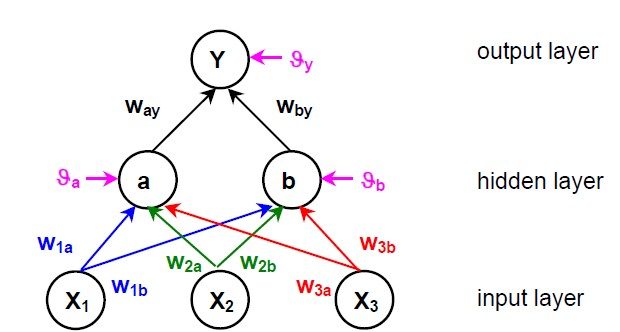
\includegraphics[width=0.45\textwidth]{Images/ArtificialNeuron.JPG} 
    \caption{Multilayer perceptron \cite{kaestner:SCANN}} 
    \label{fig:ArtificialNeuron} 
\end{figure}

\par In the Figure \ref{fig:ArtificialNeuron} it can be seen how the inputs are passed to the hidden layer, for this, the input is multiplied by a certain coefficient before entering the hidden stage, to later add a weight to it, process the data and go through the same process to pass it to the output layer \cite{kaestner:SCANN}.

\begin{figure}[H] 
    \centering
    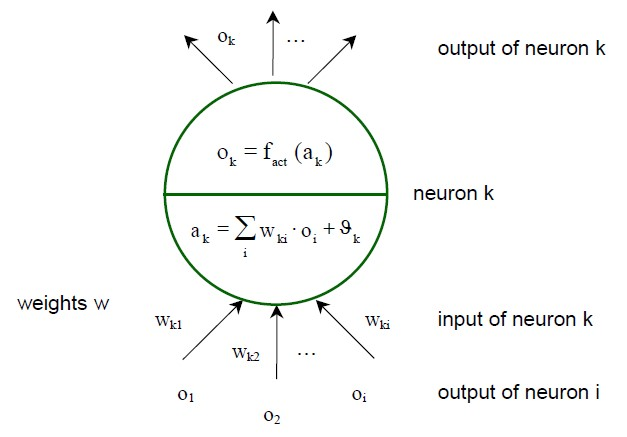
\includegraphics[width=0.45\textwidth]{Images/ArtificialNeuronProcess.JPG} 
    \caption{Artificial neuron \cite{kaestner:SCANN}} 
    \label{fig:ArtificialNeuronProcess} 
\end{figure}

\par Figure \ref{fig:ArtificialNeuronProcess} shows graphically the process described above.

\par Multilayer perceptrons, depending on their structure, can also be classified in 3 different ways. Feed forward if neurons only point to the next layer as in Figure \ref{fig:FeedForward}, lateral if neurons in the same layer can also communicate with each other as in Figure \ref{fig:Lateral}, and recurrent if different layers can interact with each other as in Figure \ref{fig:Recurrent}  \cite{kaestner:SCANN}. 

\begin{figure}[H] 
    \centering
    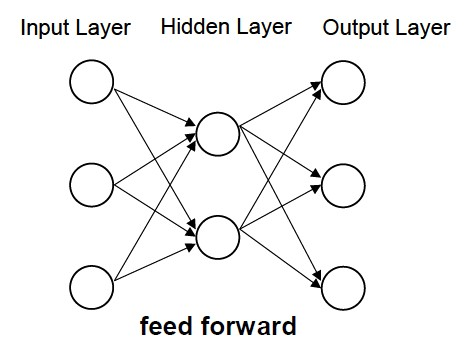
\includegraphics[width=0.35\textwidth]{Images/FeedForward.JPG} 
    \caption{Artificial neural networks in a feed forward configuration \cite{kaestner:SCANN}} 
    \label{fig:FeedForward} 
\end{figure}

\begin{figure}[H] 
    \centering
    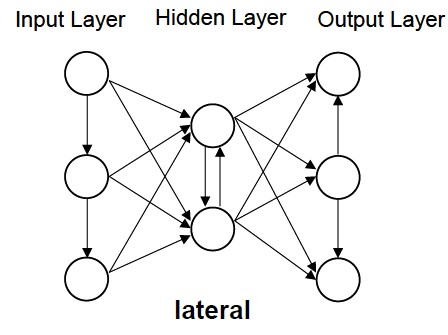
\includegraphics[width=0.35\textwidth]{Images/Lateral.JPG} 
    \caption{Artificial neural networks in a lateral configuration \cite{kaestner:SCANN}} 
    \label{fig:Lateral} 
\end{figure}

\begin{figure}[H] 
    \centering
    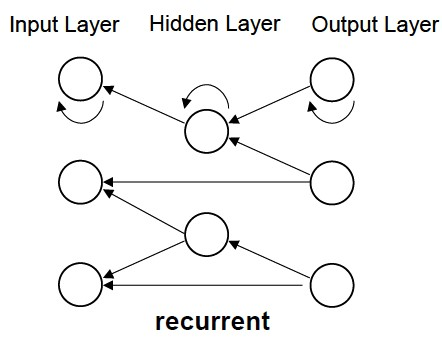
\includegraphics[width=0.35\textwidth]{Images/Recurrent.JPG} 
    \caption{Artificial neural networks in a recurrent configuration \cite{kaestner:SCANN}} 
    \label{fig:Recurrent} 
\end{figure}

\subsubsection{Multi-Layer Perceptron (MLP) Design} 
\par For the design of a MLP in the selected software, DataEngine, it is necessary to first define some parameters related to the structure and the way of processing the information. First, it is important to determine the strategy for determining the values of the weights, also known as Backpropagation with Momentum-term \cite{kaestner:SCANN}. Subsequently, it is necessary to define the Bias neuron, which is the assignment of a threshold value that acts as an additional neuron, providing the interpolation capability \cite{kaestner:SCANN}. Next, it is necessary to define the Symmetry Breaking, which is the initialization of the variables with random values to avoid errors of identical values \cite{kaestner:SCANN}. Then, it is also necessary to define Weight Decay, which is the process to homogenize the distribution of weights, in order to avoid critical nodes that have too much weight in the final result \cite{kaestner:SCANN}. And finally, it is necessary to define Pruning, which is the process of eliminating non-relevant connections and simplifying the model \cite{kaestner:SCANN}.



\subsection{Markov Model} 

\par However, one of the main components of this project is the Markov model. Which, in a nutshell, is a model that, depending on the stress conditions of a system, is able to estimate the lifetime. To understand the model, it is necessary to first define some concepts, such as reliability assessment, which is the prediction of system failures based on probabilities \cite{kaestner:Mark}. It is also important to define reliability, which is the description of system availability and the factors that influence it, such as functional capability, maintainability, etc \cite{kaestner:Mark}.
\par Another important concept is availability, which is the probability that the system will be in a functional state at a defined time \cite{kaestner:Mark}. Non-availability is the complementary value to this and permanent availability is the parameter for the description of a repairable system \cite{kaestner:Mark}.
\par Going into a little more detail, the Markov model starts from the idea that any system as in Figure \ref{fig:BinaryModel} can be found in one of two states, either intact or defect, where to pass from one to the other there is a probability of failure or repair \cite{kaestner:Mark}.

\begin{figure}[H] 
    \centering
    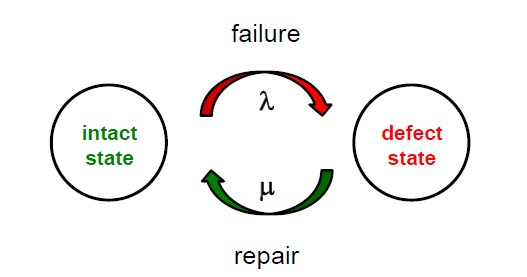
\includegraphics[width=0.4\textwidth]{Images/BinaryModelSystemState.JPG} 
    \caption{Binary model system state \cite{kaestner:Mark}} 
    \label{fig:BinaryModel} 
\end{figure}



\subsubsection{Failure rate}

\par The probability of failure describes the time that a non-faulty system, after a time t, will fail \cite{kaestner:Mark}. This can be calculated by dividing the density of the probability of failure by the probability of survival or reliability \cite{kaestner:Mark}.

\begin{figure}[H] 
    \centering
    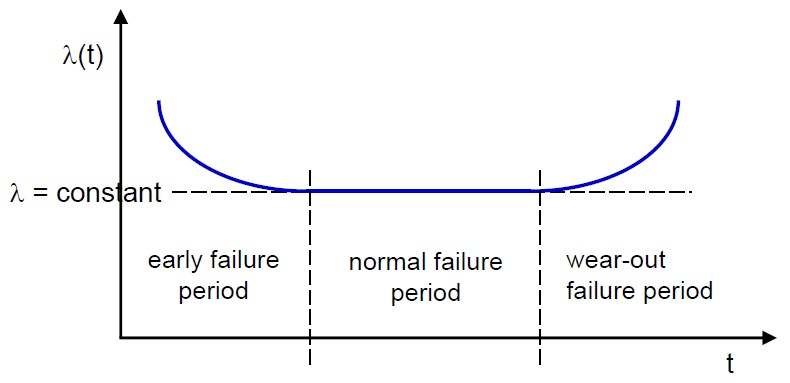
\includegraphics[width=0.6\textwidth]{Images/BathCurve.JPG} 
    \caption{Failure rate curve \cite{kaestner:Mark}} 
    \label{fig:BathCurve} 
\end{figure}

\par As can be seen in Figure \ref{fig:BathCurve} the failure probability is a function of time describing a bath-tub curve \cite{kaestner:Mark} This curve can be divided into three main phases, the first one of early failure where, due to the early use of elements, they tend to fail, but then show a decline in this failure \cite{kaestner:Mark}. A second stage of normal failure where the highest reliability of the system is reached and this is the desired period of operation \cite{kaestner:Mark}. Finally, there is the wear-out phase where there is a systematic failure due to aging, fatigue, wear-out of the components and it is the phase where maintenance or corrective measures should be provided \cite{kaestner:Mark}. The life time of a component or system can also be obtained or visualized from the graph . Some of the most important characteristics of the probability of failure are that it has a continuous distribution over the lifetime, this being, mathematically, an exponential distribution \cite{kaestner:Mark}.

$$ \textrm{Failure rate} =  \lambda $$
$$ \textrm{Repair rate} =  \mu $$

\begin{itemize}

\item Reliability or probability of survival $ R(t) $
\begin{equation}
R(t) = e^{-\lambda t}
\label{eq:Rt1}
\end{equation}

\item Probability of failure $F(t)$
\begin{equation}
F(t) = 1 - e^{-\lambda t}
\label{eq:Ft1}
\end{equation}

\item Life time $\overline{T}$
\begin{equation}
\overline{T} = \int_{0}^{\infty} R(t) \,dt = \frac{1}{\lambda}
\label{eq:T1}
\end{equation}

\end{itemize}

\begin{figure}[H] 
    \centering
    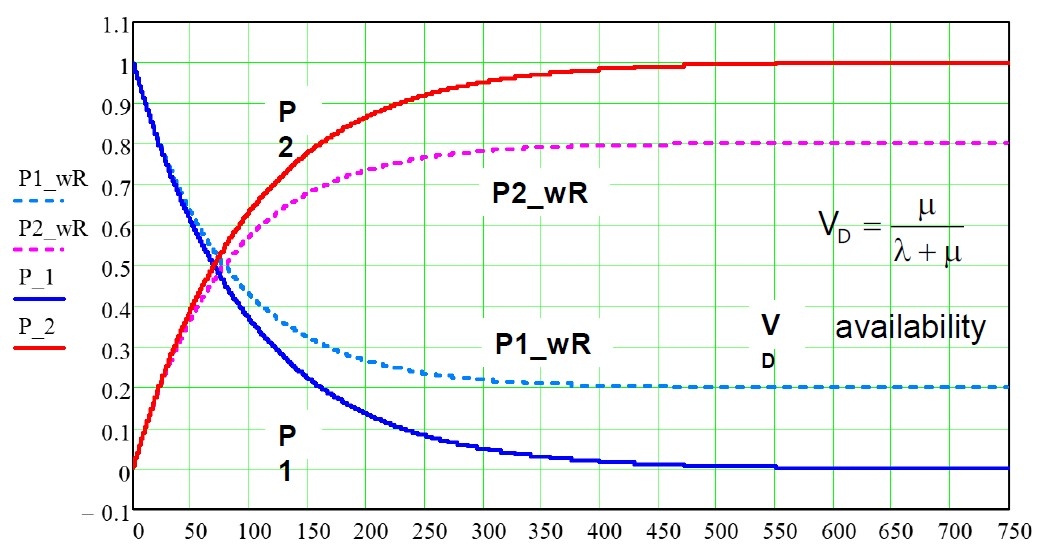
\includegraphics[width=0.6\textwidth]{Images/FailurevSurvival.JPG} 
    \caption{Failure vs survival rate on a single component w/without repair \cite{kaestner:Mark}} 
    \label{fig:FailurevSurvival} 
\end{figure}



\subsubsection{Redundancy}
\par Another important concept to take into account is redundancy, which is, in general terms, the arrangement of multiple elements in the same form \cite{kaestner:Mark}. This provides a system with protection against random independent failures \cite{kaestner:Mark}.

\begin{figure}[H] 
    \centering
    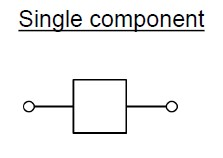
\includegraphics[width=0.3\textwidth]{Images/SingleComponent.JPG} 
    \caption{Single component \cite{kaestner:Mark}} 
    \label{fig:SingleComponent} 
\end{figure}



\begin{figure}[H] 
    \centering
    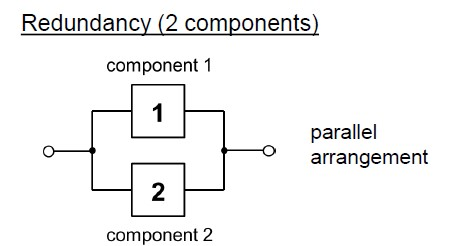
\includegraphics[width=0.5\textwidth]{Images/TwoComponents.JPG} 
    \caption{Two components in parallel \cite{kaestner:Mark}} 
    \label{fig:TwoComponents} 
\end{figure}

$$\textrm{Single component}$$
$$W(a)=W(e)=p=0.9$$
$$\textrm{Two components}$$
$$W(a)=1-\prod_{i=1}^{2} (1-p_{i})$$
$$W(A)=1-(1-2p+p^2) $$
\begin{equation}
W(a)=2p-p^2=0.99
\end{equation}

\par As can be seen in Figures \ref{fig:SingleComponent} and \ref{fig:TwoComponents}, thanks to redundancy it is possible to increase the reliability probability of a component with a reliability of 90\% by an additional 9\% \cite{kaestner:Mark}.

\par This translated into the equations of \ref{eq:Rt1}, \ref{eq:Ft1} and \ref{eq:T1} gives that the lifetime of a system can be increased by up to 50\% with respect to the original model \cite{kaestner:Mark}.

\begin{itemize}

\item Reliability or probability of survival $ R(t) $
\begin{equation}
R(t) = 1- F(t)=2e^{-\lambda t}-e^{-2 \lambda t}
\label{eq:Rt2}
\end{equation}

\item Probability of failure $F(t)$
\begin{equation}
F(t) = (1 - e^{-\lambda t})^2 = 1-2e^{-\lambda t}+e^{-2 \lambda t}
\label{eq:Ft2}
\end{equation}

\item Life time $\overline{T}$
\begin{equation}
\overline{T} = \int_{0}^{\infty} R(t) \,dt = \frac{2}{\lambda} - \frac{1}{2 \lambda}=1.5 \frac{1}{\lambda}
\label{eq:T2}
\end{equation}

\end{itemize}



\subsubsection{Markov model: Evaluation of reliability}
\par Within the Markov model, the probabilities of the states of the binary model are used to evaluate the probability of the state in which the system is found \cite{kaestner:Mark}. The Markov model is governed by the probability of failure and repair, since with these a vector of differential equations of order k is constructed, where k is the number of states of the system \cite{kaestner:Mark}.

\begin{figure}[H] 
    \centering
    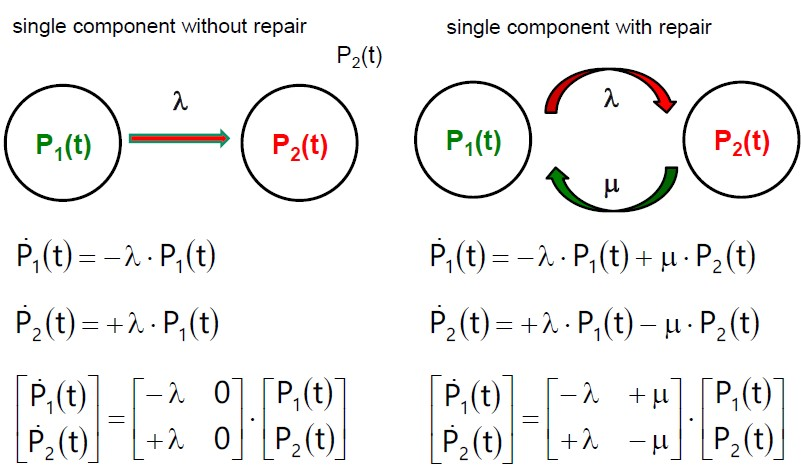
\includegraphics[width=0.6\textwidth]{Images/Markov.JPG} 
    \caption{Markov model \cite{kaestner:Mark}} 
    \label{fig:Markov} 
\end{figure}




\subsection{Methodology}
\par Regarding the process to be followed for the construction of the multilayer perceptron and its use in the Markov model. For the construction of the MLP, it is necessary to first pre-process the data or filter it from any erroneous data. Then a second filtering stage is required to separate the data for testing and training. Then it is required to first train the MLP with pruning in order to determine a more optimized model, apply the optimizations, remove pruning and train it, then test the test data and evaluate if the results are satisfactory. Finally, it is necessary to implement the MLP in a simulation software with the connections configured according to the Markov model, simulate, obtain the results, analyze them and issue a conclusion. 





%========================%
%    Data-preprocessing  %
%========================%

\newpage
\section{Data pre-processing}

\par As already mentioned, we are going to start with an initial data set, which, being directly collected from the measurement system, may or may not come with errors. The origin of these errors may well be directly the sensor, which made some erroneous detection by some internal error, these errors will be called measuring errors. Another possible origin is the processing of the sensor signal and they manifest themselves in the form of out-of-range values or sensor defect. And the last possible origin are duplicate or redundant values that only hinder the processing



\subsection{Atypical values}

\par As already mentioned, we are going to start with a data set, see table \ref{table:InitialData} in appendix \ref{appendix:tables}. These data were taken directly from the measurement system, so a first filtering is required in order to deliver only valid data to the next stage. To better visualize what we are talking about, in the Figure \ref{fig:RawData2} and \ref{fig:RawData1} it can be seen how there are certain values that stand out for having a completely different behavior from the rest and that if processed would result in an inconsistent model.

\begin{figure}[H] 
    \centering
    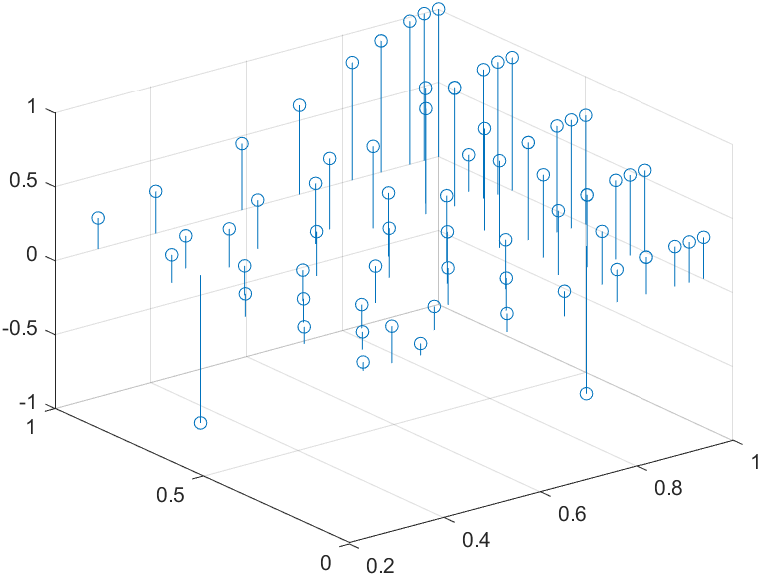
\includegraphics[width=0.5\textwidth]{Images/RawData2.JPG} 
    \caption{Raw data visualization} 
    \label{fig:RawData2} 
\end{figure}

\begin{figure}[H] 
    \centering
    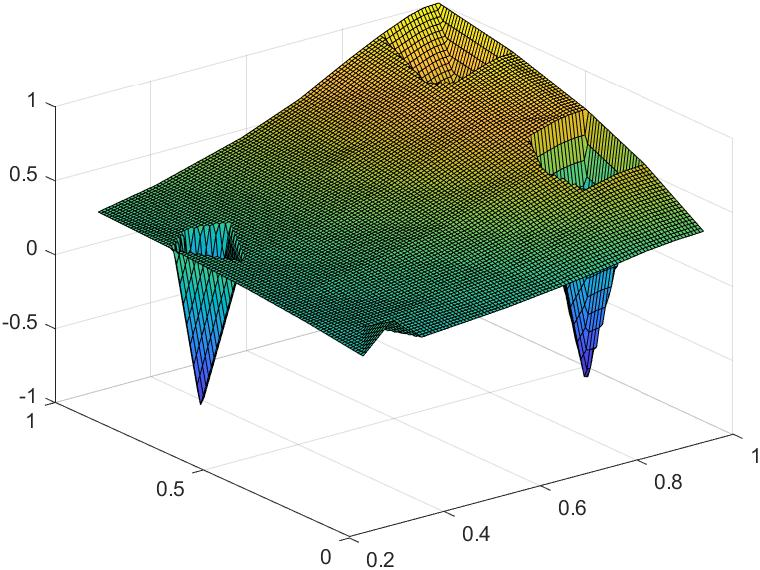
\includegraphics[width=0.5\textwidth]{Images/RawData1.JPG} 
    \caption{Raw data on a mesh-grid} 
    \label{fig:RawData1} 
\end{figure}


\subsubsection{Sensor defect}

\par The purpose of this first filter is to eliminate all those values that are physically impossible to occur in real life. These can be easily detected by the out-of-range values, in this case, the measurements being between 0 and 1, 2 values with -1 will be eliminated. The remaining values give the behavior of Figure \ref{fig:FirstFilter1}.

\begin{figure}[H] 
    \centering
    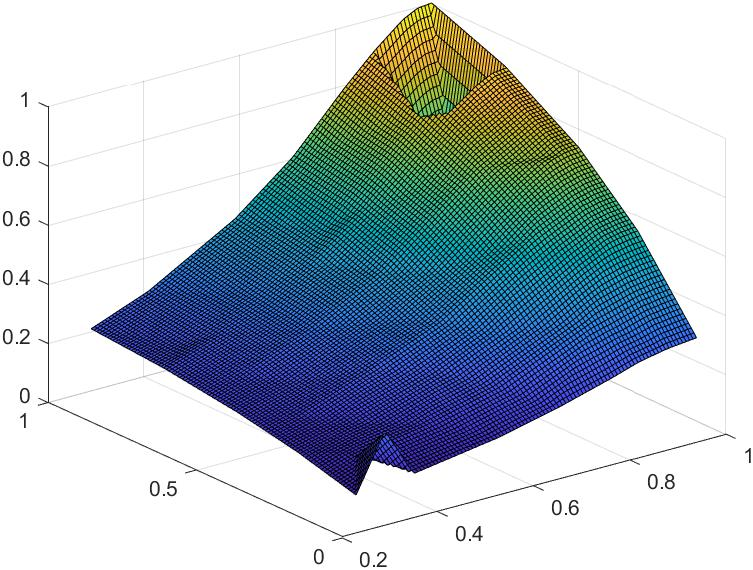
\includegraphics[width=0.5\textwidth]{Images/FirstFilter1.JPG} 
    \caption{Data after first filter} 
    \label{fig:FirstFilter1} 
\end{figure}



\par As can be seen, in spite of having eliminated the most important outliers, the graph still has points where the general trend has a sudden change, but this will be analyzed later.

\subsubsection{Redundant data}

\noindent This next stage of filtering is a little more complicated to visualize graphically, as most of the graphing software eliminates these values by itself and it is only possible to detect them manually. For the given data set, there are 2 measurements for the same value of X1 = 0.88. Therefore, it will be decided to eliminate 5 repeated values, which despite having more significant figures, do not bring more precision.

\subsubsection{Measuring errors}

\par Finally, the Figure \ref{fig:FirstFilter1} shows how there are two values that bring an abrupt change to the general behavior of the data. To eliminate them, the behavior of the data is simply analyzed and if a value that changes the gradient is found, it will be eliminated. After running the code, 2 data were removed and the remaining data are shown in Figures \ref{fig:Processed2} and \ref{fig:Processed1} .

\begin{figure}[H] 
    \centering
    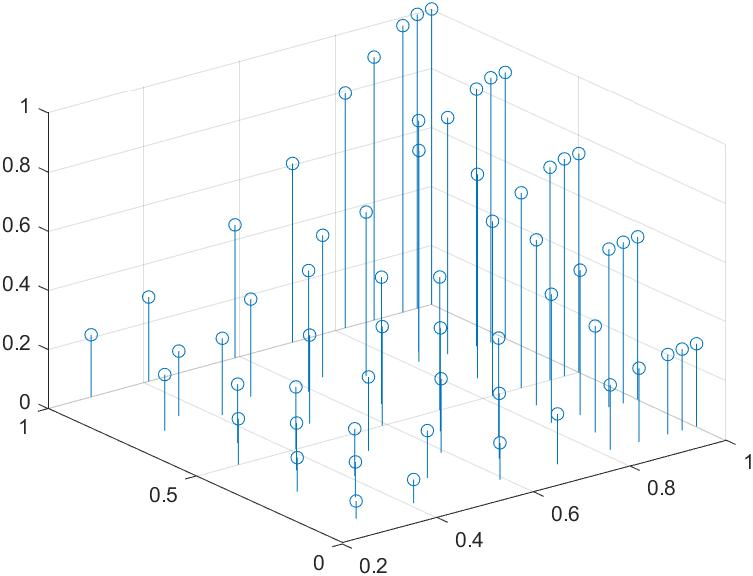
\includegraphics[width=0.5\textwidth]{Images/ProcessedData2.JPG} 
    \caption{Final processed data graph} 
    \label{fig:Processed2} 
\end{figure}

\begin{figure}[H] 
    \centering
    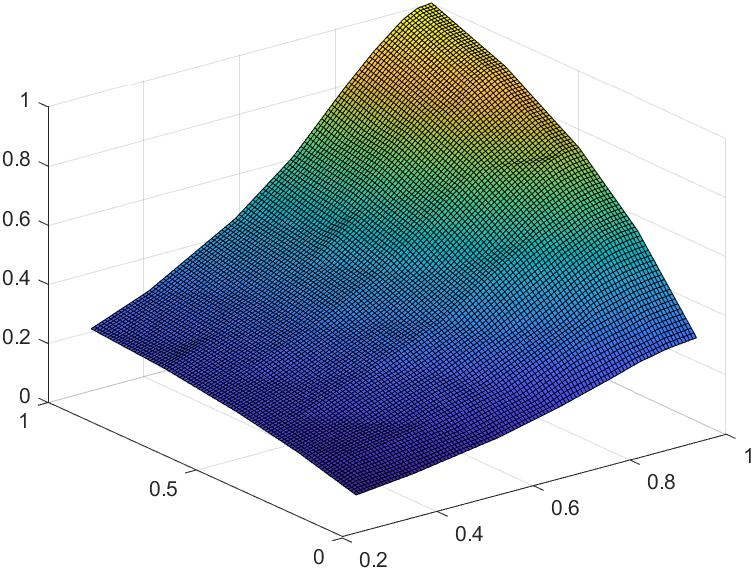
\includegraphics[width=0.5\textwidth]{Images/ProcessedData1.JPG} 
    \caption{Final processed data mesh-grid} 
    \label{fig:Processed1} 
\end{figure}





%========================%
%     Data-preparation   %
%========================%
\newpage
\section{Data preparation}

\par For both the pre-processing and data preparation sections, the Code \ref{code:MatLab} in Appendix \ref{appendix:codes} was designed, programmed and tested. This code performed the filtering described in the previous section, as well as the separation of the data into two sets, one for training and one for testing. 

\subsection{Considerations}

\par For this stage we sought to implement a process that would guarantee not only a maximum error within the limits of 3\% for MLP training and testing, but that would also be flexible and allow several possible training and testing sets. For this purpose, a variable called tolerance was created, which, in short, sets aside the maximum and minimum values minus or plus the tolerance and leaves the remaining data available for random selection, where the user determines the amount of data for testing. 

\subsection{Data}

\par In the case of this project, a tolerance of 20\% was selected with a test data set of maximum 20 data. The program ran, performed the filtering and separation of the data, to finally deliver the two data sets.

\subsubsection{Training data}

\par As can be seen, the data set obtained contains the maximum and minimum data minus or plus the tolerance of the three variables, X1, X2 and Y. This decision will ensure that the largest gradients or groups of data that would provide a greater error are already considered and therefore the resulting error is minimal. There is a total of 41 data for training.

\begin{longtable}[c]{|c|c|c|}
\hline
X1   & X2   & Y     \\ \hline
\endfirsthead
%
\multicolumn{3}{c}%
{{\bfseries Table \thetable\ continued from previous page}} \\
\endhead
%
0.29 & 0.1  & 0.06  \\ \hline
0.41 & 0.1  & 0.08  \\ \hline
0.29 & 0.3  & 0.115 \\ \hline
0.59 & 0.1  & 0.125 \\ \hline
0.29 & 0.5  & 0.155 \\ \hline
0.71 & 0.1  & 0.17  \\ \hline
0.29 & 0.75 & 0.19  \\ \hline
0.29 & 1    & 0.21  \\ \hline
0.82 & 0.1  & 0.22  \\ \hline
0.88 & 0.1  & 0.25  \\ \hline
0.94 & 0.1  & 0.27  \\ \hline
0.97 & 0.1  & 0.275 \\ \hline
1    & 0.1  & 0.28  \\ \hline
0.41 & 1    & 0.285 \\ \hline
0.59 & 1    & 0.45  \\ \hline
0.88 & 0.3  & 0.49  \\ \hline
0.94 & 0.3  & 0.535 \\ \hline
0.97 & 0.3  & 0.545 \\ \hline
1    & 0.3  & 0.55  \\ \hline
0.71 & 1    & 0.605 \\ \hline
0.88 & 0.5  & 0.66  \\ \hline
0.94 & 0.5  & 0.72  \\ \hline
0.97 & 0.5  & 0.735 \\ \hline
1    & 0.5  & 0.74  \\ \hline
0.82 & 1    & 0.795 \\ \hline
0.88 & 0.75 & 0.8   \\ \hline
0.94 & 0.75 & 0.87  \\ \hline
0.88 & 1    & 0.89  \\ \hline
0.97 & 0.75 & 0.895 \\ \hline
1    & 0.75 & 0.9   \\ \hline
0.94 & 1    & 0.97  \\ \hline
0.97 & 1    & 0.995 \\ \hline
1    & 1    & 1     \\ \hline
0.35 & 0.2  & 0.12  \\ \hline
0.35 & 0.4  & 0.16  \\ \hline
0.41 & 0.3  & 0.16  \\ \hline
0.5  & 0.2  & 0.16  \\ \hline
0.35 & 0.6  & 0.2   \\ \hline
0.41 & 0.5  & 0.21  \\ \hline
0.35 & 0.8  & 0.22  \\ \hline
0.65 & 0.2  & 0.22  \\ \hline
\caption{Training data set}
\label{table:TrainingData}
\end{longtable}



\subsubsection{Test data}

\par As can be seen, the data obtained for the testing are average and very standard values for the three parameters X1, X2 and Y.  All the maximum and minimum values together with the tolerance were separated, so that the separation of these data to form part of the test should not alter the general behavior of the system. There is a total of 20 data for testing.

\begin{longtable}[c]{|c|c|c|}
\hline
\textbf{X1} & \textbf{X2} & \textbf{Y} \\ \hline
\endfirsthead
%
\multicolumn{3}{c}%
{{\bfseries Table \thetable\ continued from previous page}} \\
\endhead
%
0.5         & 0.4         & 0.25       \\ \hline
0.59        & 0.3         & 0.25       \\ \hline
0.41        & 0.75        & 0.26       \\ \hline
0.5         & 0.6         & 0.3        \\ \hline
0.5         & 0.8         & 0.33       \\ \hline
0.59        & 0.5         & 0.335      \\ \hline
0.71        & 0.3         & 0.335      \\ \hline
0.65        & 0.4         & 0.35       \\ \hline
0.85        & 0.2         & 0.36       \\ \hline
0.59        & 0.75        & 0.41       \\ \hline
0.65        & 0.6         & 0.43       \\ \hline
0.82        & 0.3         & 0.435      \\ \hline
0.71        & 0.5         & 0.45       \\ \hline
0.65        & 0.8         & 0.48       \\ \hline
0.71        & 0.75        & 0.555      \\ \hline
0.85        & 0.4         & 0.56       \\ \hline
0.82        & 0.5         & 0.59       \\ \hline
0.85        & 0.6         & 0.69       \\ \hline
0.82        & 0.75        & 0.715      \\ \hline
0.85        & 0.8         & 0.78       \\ \hline
\caption{Test data set}
\label{table:TestData}
\end{longtable}





%========================%
%        MLP design      %
%========================%

\newpage

\section{MLP design}

\par As already mentioned, the design of an MLP requires the definition of several variables. These variables range from the number of inputs and outputs, the number of hidden layers, back-propagation, momentum, etc.... The definition of these variables is of vital importance, because as mentioned in the methodology, they will allow us to calculate a first model with pruning, which will give us the optimal number of connections, to later make a second model without pruning that really optimally models the data set without losing interpolation capacity.The overall goal that must be achieved is to create a MLP with a maximum error lower than $\pm 3\%$. In Appendix \ref{appendix:steps} it can be seen the whole design process within the software's windows.

\subsection{Parameters}

\par There are some parameters that will not change between the models with and without pruning, these being the learning parameters:

\begin{itemize}
\item Learning parameters

\begin{longtable}[c]{|c|c|c|c|}
\hline
                      & \textbf{First hidden layer} & \textbf{Second hidden layer} & \textbf{Output layer} \\ \hline
\endfirsthead
%
\multicolumn{4}{c}%
{{\bfseries Table \thetable\ continued from previous page}} \\
\endhead
%
\textbf{Learn ratio}  & 0,1                         & 0,1                          & 0,9999999             \\ \hline
\textbf{Momentum}     & 0,1                         & 0,1                          & 0,9999999             \\ \hline
\textbf{Weight-decay} & 0,1                         & 0,1                          & 0,9999999             \\ \hline
\caption{Learning parameters}
\end{longtable}



\item Weights initialization 

\begin{longtable}[c]{|l|l|}
\hline
\textbf{Lower limit:}   & -0,1       \\ \hline
\endfirsthead
%
\multicolumn{2}{c}%
{{\bfseries Table \thetable\ continued from previous page}} \\
\endhead
%
\textbf{Upper limit:}   & 0,1        \\ \hline
\textbf{Initial value:} & 1234567890 \\ \hline
\caption{Weights initialization}
\end{longtable}



\item Stop conditions

\begin{longtable}[c]{|c|c|}
\hline
\textbf{\textless max. training error}        & 0,0001                         \\ \hline
\endfirsthead
%
\multicolumn{2}{c}%
{{\bfseries Table \thetable\ continued from previous page}} \\
\endhead
%
\textbf{\textless{}RMS training error}        & 0,0001                         \\ \hline
\textbf{\textless{}max. training error}       & 0,0001                         \\ \hline
\textbf{\textless{}RMS training error}        & 0,0001                         \\ \hline
\textbf{number of iterations is divisible by} & 100.000                        \\ \hline
\textbf{iterations}                           & 100.000                        \\ \hline
\textbf{error measurement}                    & 0,9 RMS error + 0,1 max. error \\ \hline
\textbf{Based on}                             & test error                     \\ \hline
\caption{Stop conditions}
\end{longtable}

\end{itemize}

\par As mentioned in the methodology, the MLP development process requires a first design phase with pruning and a second phase without pruning. However, both share the same data and the parameters described above. The main differences come from the network structure itself and the learning process used.

\subsubsection{Before pruning}

\par Before pruning, the network structure must have more connections than the data used. So if by default you have two inputs and one output, that means that the other connections must come from the hidden layers, for this reason, it was also decided to use two hidden layers instead of one, because if that had been done, the hidden layer would have been very large compared to its neighbors. 

\begin{longtable}[c]{|c|c|c|}
\hline
\textbf{}                     & \textbf{Number of neurons} & \textbf{Transfer function} \\ \hline
\endfirsthead
%
\multicolumn{3}{c}%
{{\bfseries Table \thetable\ continued from previous page}} \\
\endhead
%
\textbf{Input:}               & 2                          & Linear                     \\ \hline
\textbf{First hidden layer:}  & 6                          & Tanh                       \\ \hline
\textbf{Second hidden layer:} & 5                          & Tanh                       \\ \hline
\textbf{Output:}              & 1                          & Linear                     \\ \hline
\caption{Architecture with pruning}
\end{longtable}

\begin{figure}[H] 
    \centering
    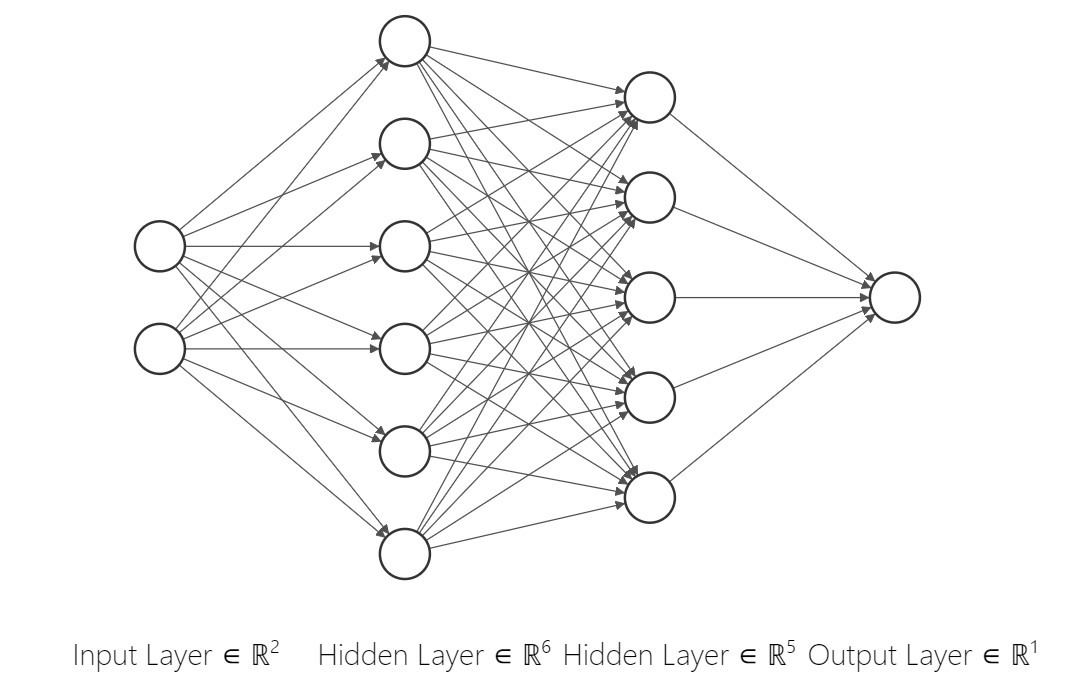
\includegraphics[width=0.8\textwidth]{Images/Photos/GraphWP.JPG} 
    \caption{Graph of artificial neural network } 
    \label{fig:GraphWP} 
\end{figure}

\par Finally, with respect to the main topic of the section, in the learning process pruning had to be activated along with certain parameters for it, like threshold, or time constant, so the algorithm can determine which connections to eliminate. Once run, the optimal number of connections was obtained, in this case only 9 connections are really necessary. This structure was then applied to the next model and optimized. 

\begin{longtable}[c]{|c|c|}
\hline
\textbf{Process}               & Backpropagation     \\ \hline
\endfirsthead
%
\multicolumn{2}{c}%
{{\bfseries Table \thetable\ continued from previous page}} \\
\endhead
%
\textbf{Momentum}              & ON                  \\ \hline
\textbf{Weight-decay}          & ON                  \\ \hline
\textbf{Learning strategy}     & Single step (delta) \\ \hline
\textbf{Presentation sequence} & Sequential          \\ \hline
\textbf{Pruning}               & ON                  \\ \hline
\textbf{Relevance threshold}   & 0,02                \\ \hline
\textbf{Time constant}         & 10                  \\ \hline
\caption{Learning process with pruning}
\end{longtable}


\par Once all the variables were set in the DataEngine software, the results shown in Figure \ref{fig:BeforePruning1} and \ref{fig:BeforePruning2} were obtained. As can be seen in them, the maximum and minimum errors, although they come from a single data, are greater than expected and therefore exceed the imposed limit of 3\% as maximum. Nevertheless, since the most optimal model should have 9 connections, this adjustment will be made to check if the model has improved. Also the error graph shows how this varied.

\begin{figure}[H] 
    \centering
    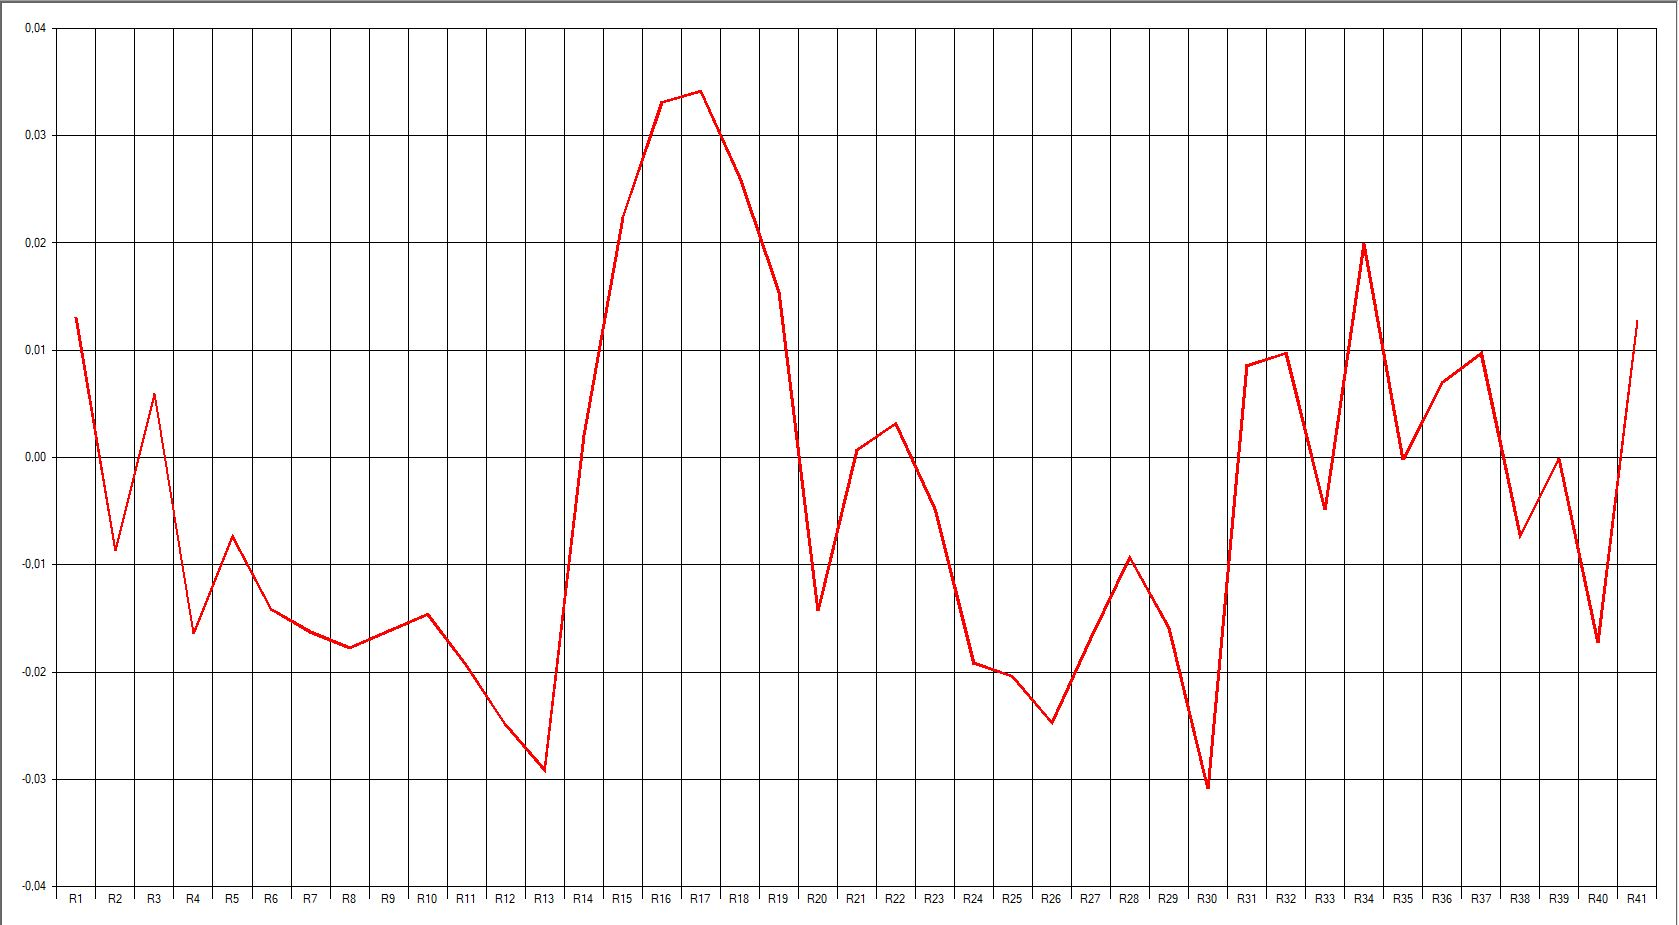
\includegraphics[width=0.8\textwidth]{Images/Photos/ErrorWP.JPG} 
    \caption{Error development for network with pruning} 
    \label{fig:ErrorWP} 
\end{figure}

\begin{figure}[H] 
    \centering
    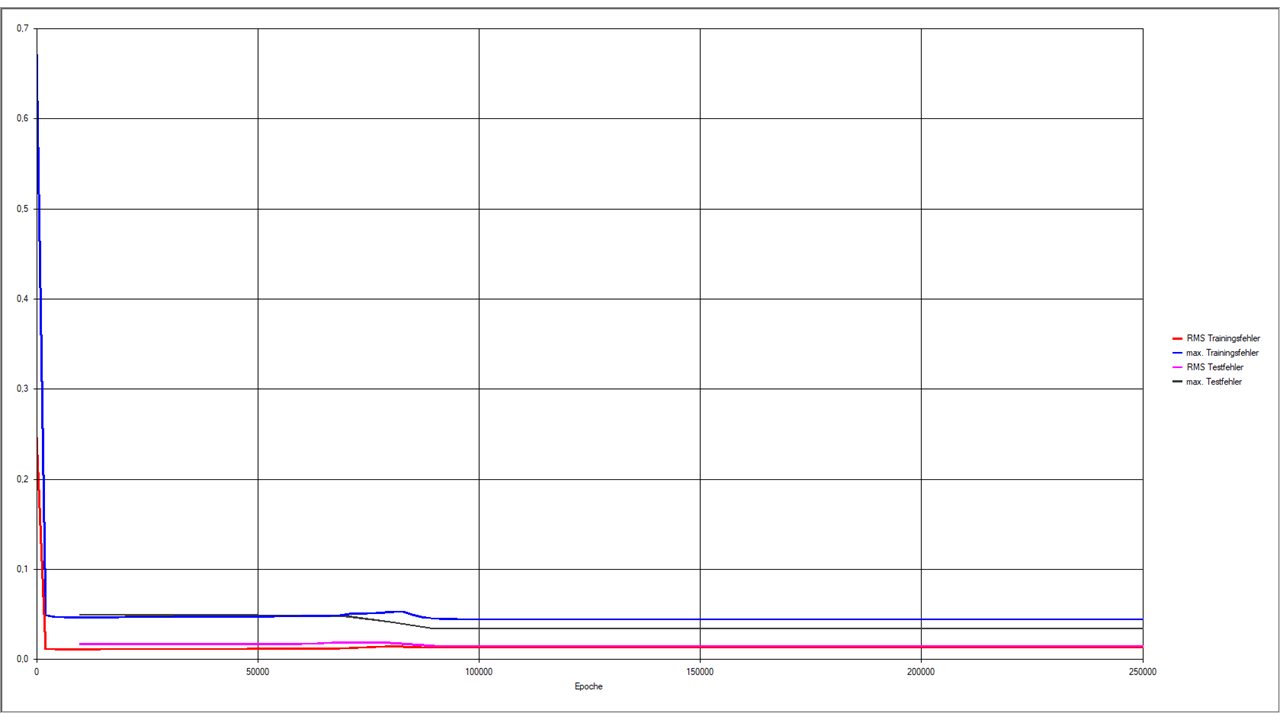
\includegraphics[width=0.8\textwidth]{Images/Fotos/Diapositiva5.PNG} 
    \caption{Results before optimization} 
    \label{fig:BeforePruning1} 
\end{figure}

\begin{figure}[H] 
    \centering
    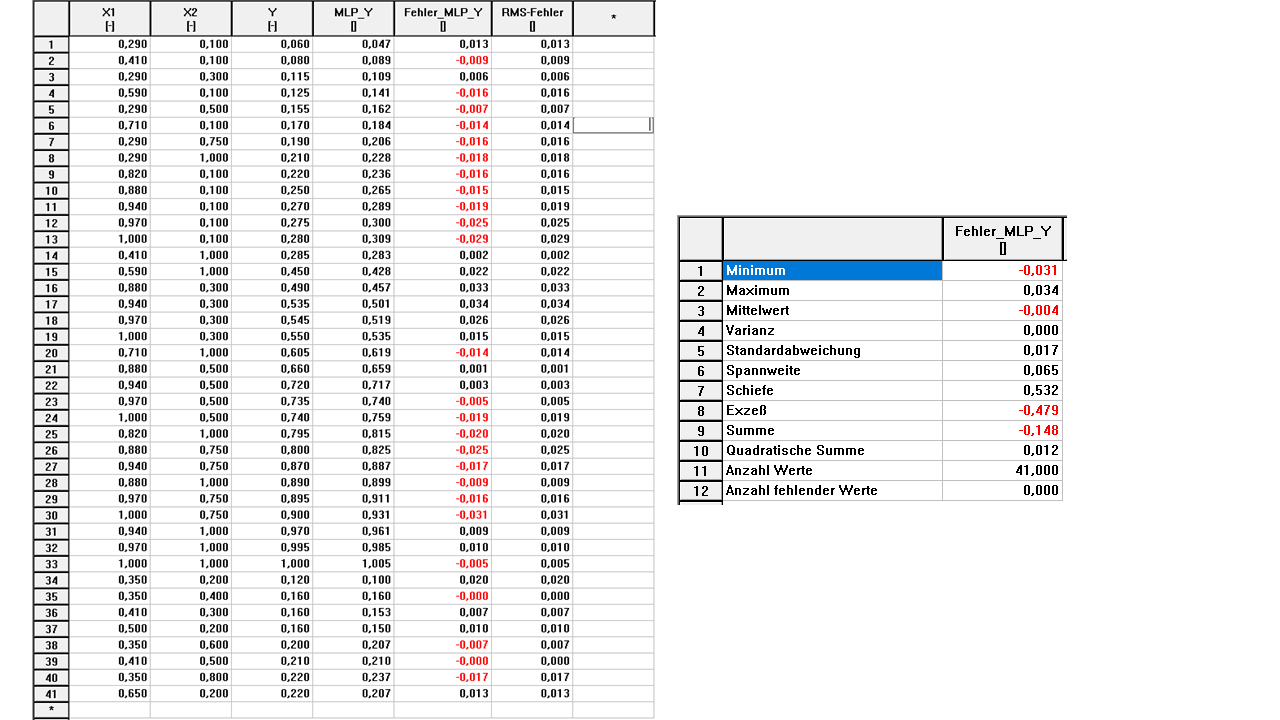
\includegraphics[width=1.0\textwidth]{Images/Fotos/Diapositiva6.PNG} 
    \caption{Error scope before optimization} 
    \label{fig:BeforePruning2} 
\end{figure}

\par For the optimization, it is also obtained, that the most relevant connections are the following:

\begin{figure}[H] 
    \centering
    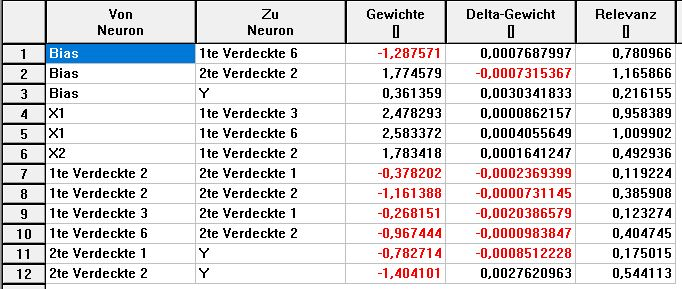
\includegraphics[width=0.8\textwidth]{Images/Photos/WeightsValuesWP.JPG} 
    \caption{Weights values with pruning} 
    \label{fig:WVWP} 
\end{figure}





\subsubsection{After pruning}

\par Once the value of connections is optimized, it is implemented in the model already created, changing the values of the hidden layers, because as mentioned, the inputs and outputs are predefined.

\begin{longtable}[c]{|c|c|c|}
\hline
\textbf{}                     & \textbf{Number of neurons} & \textbf{Transfer function} \\ \hline
\endfirsthead
%
\multicolumn{3}{c}%
{{\bfseries Table \thetable\ continued from previous page}} \\
\endhead
%
\textbf{Input:}               & 2                          & Linear                     \\ \hline
\textbf{First hidden layer:}  & 3                          & Tanh                       \\ \hline
\textbf{Second hidden layer:} & 2                          & Tanh                       \\ \hline
\textbf{Output:}              & 1                          & Linear                     \\ \hline
\caption{Architecture after pruning}
\end{longtable}

\begin{figure}[H] 
    \centering
    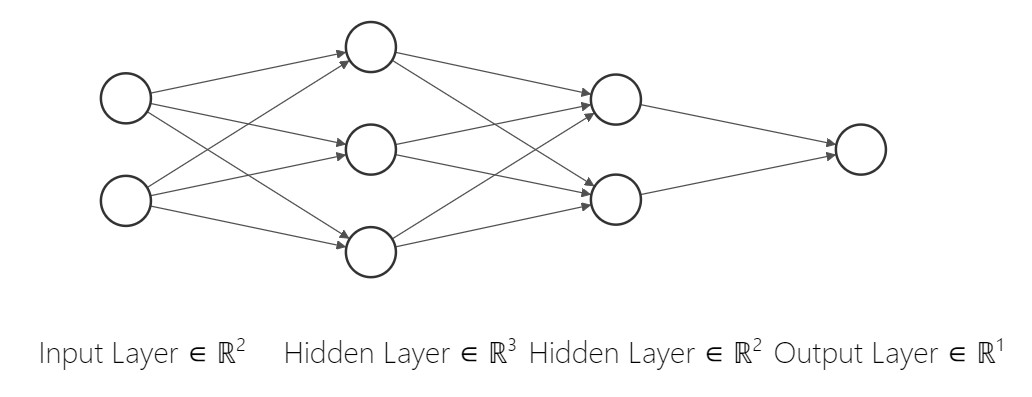
\includegraphics[width=0.8\textwidth]{Images/Photos/GraphOP.JPG} 
    \caption{Graph of artificial neural network without pruning} 
    \label{fig:GraphOP} 
\end{figure}

\par Finally, only the pruning option is deactivated to calculate the final model. 

\begin{longtable}[c]{|c|c|}
\hline
\textbf{Process}               & Backpropagation     \\ \hline
\endfirsthead
%
\multicolumn{2}{c}%
{{\bfseries Table \thetable\ continued from previous page}} \\
\endhead
%
\textbf{Momentum}              & ON                  \\ \hline
\textbf{Weight-decay}          & ON                  \\ \hline
\textbf{Learning strategy}     & Single step (delta) \\ \hline
\textbf{Presentation sequence} & Sequential          \\ \hline
\textbf{Pruning}               & OFF                 \\ \hline
\textbf{Relevance threshold}   & -                   \\ \hline
\textbf{Time constant}         & -                   \\ \hline
\caption {Learning process without pruning}
\end{longtable}

\par As can be seen in Figures \ref{fig:AfterPruning1} and \ref{fig:AfterPruning2}, the results of the training data are much more satisfactory and are within the established limit of $\pm 3\%$, as they are of -1.0\% and 1.2\%. Also the error graph showed an improvement.

\begin{figure}[H] 
    \centering
    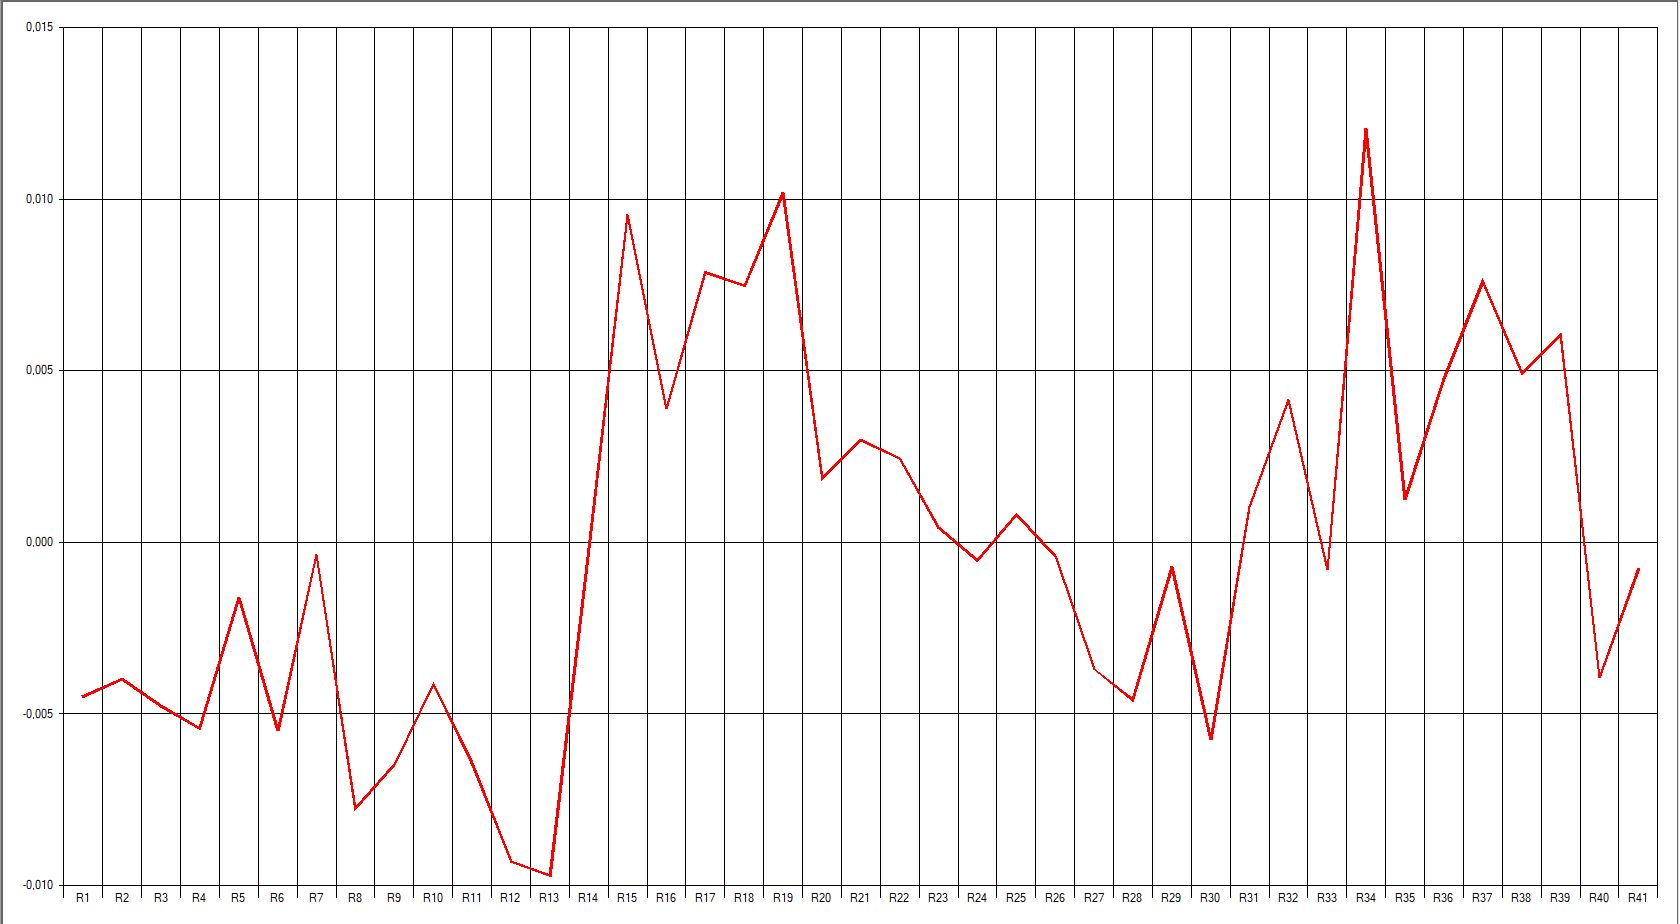
\includegraphics[width=1.0\textwidth]{Images/Photos/ErrorOP.JPG} 
    \caption{Error progression without pruning} 
    \label{fig:ErrorOP} 
\end{figure}

\begin{figure}[H] 
    \centering
    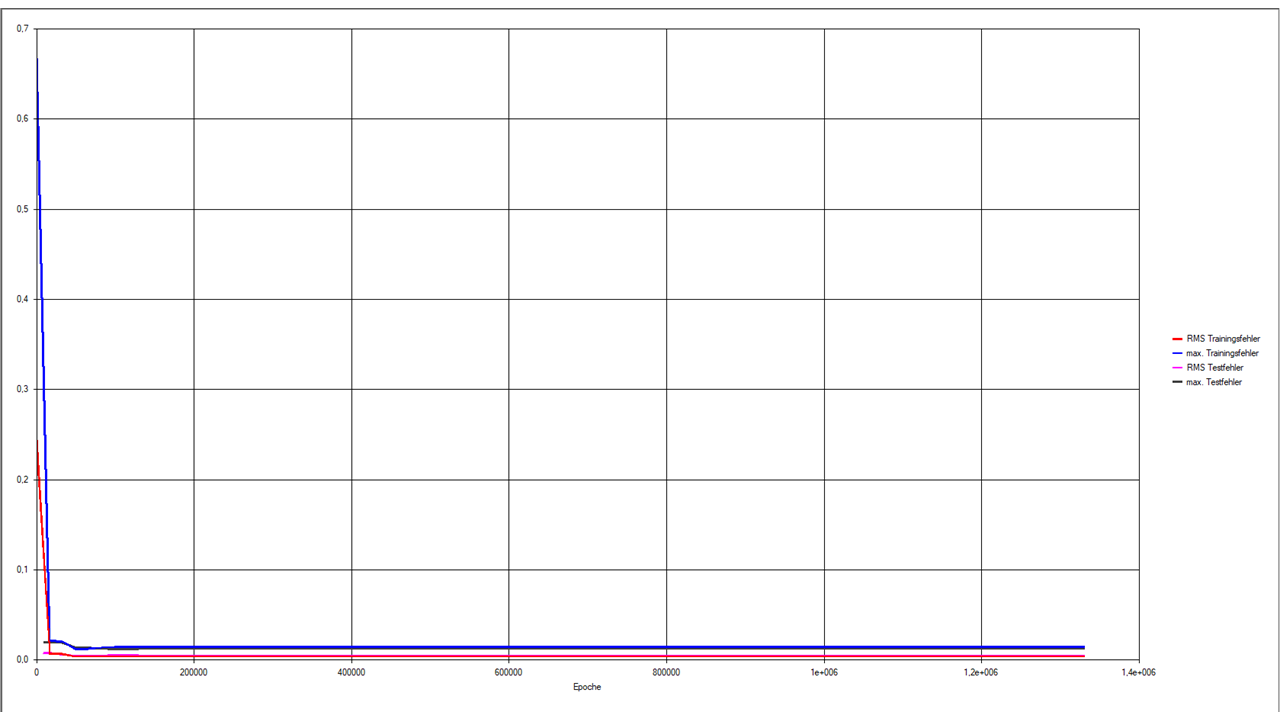
\includegraphics[width=1.0\textwidth]{Images/Fotos/Diapositiva8.PNG} 
    \caption{Results after optimization} 
    \label{fig:AfterPruning1} 
\end{figure}

\begin{figure}[H] 
    \centering
    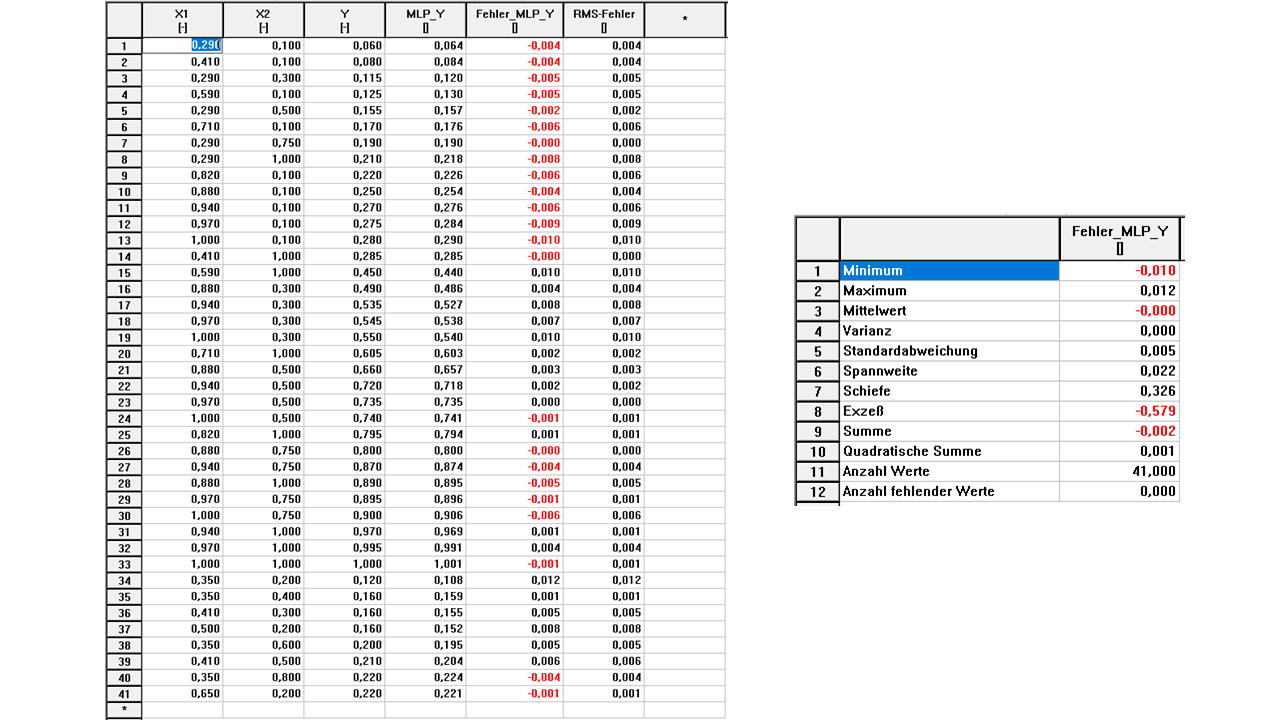
\includegraphics[width=0.95\textwidth]{Images/Fotos/Diapositiva10.PNG} 
    \caption{Error scope after optimization} 
    \label{fig:AfterPruning2} 
\end{figure}

\par Finally, with the new model, it is possible to run the training data and verify if the model is really valid or if it is necessary to make changes in the parameters. As can be seen in Figure \ref{fig:ResultsTest}, the errors and minimums are 0.3\% and 2.6\%, so they are effectively within the limit and the model is valid for the next stage. 

\begin{figure}[H] 
    \centering
    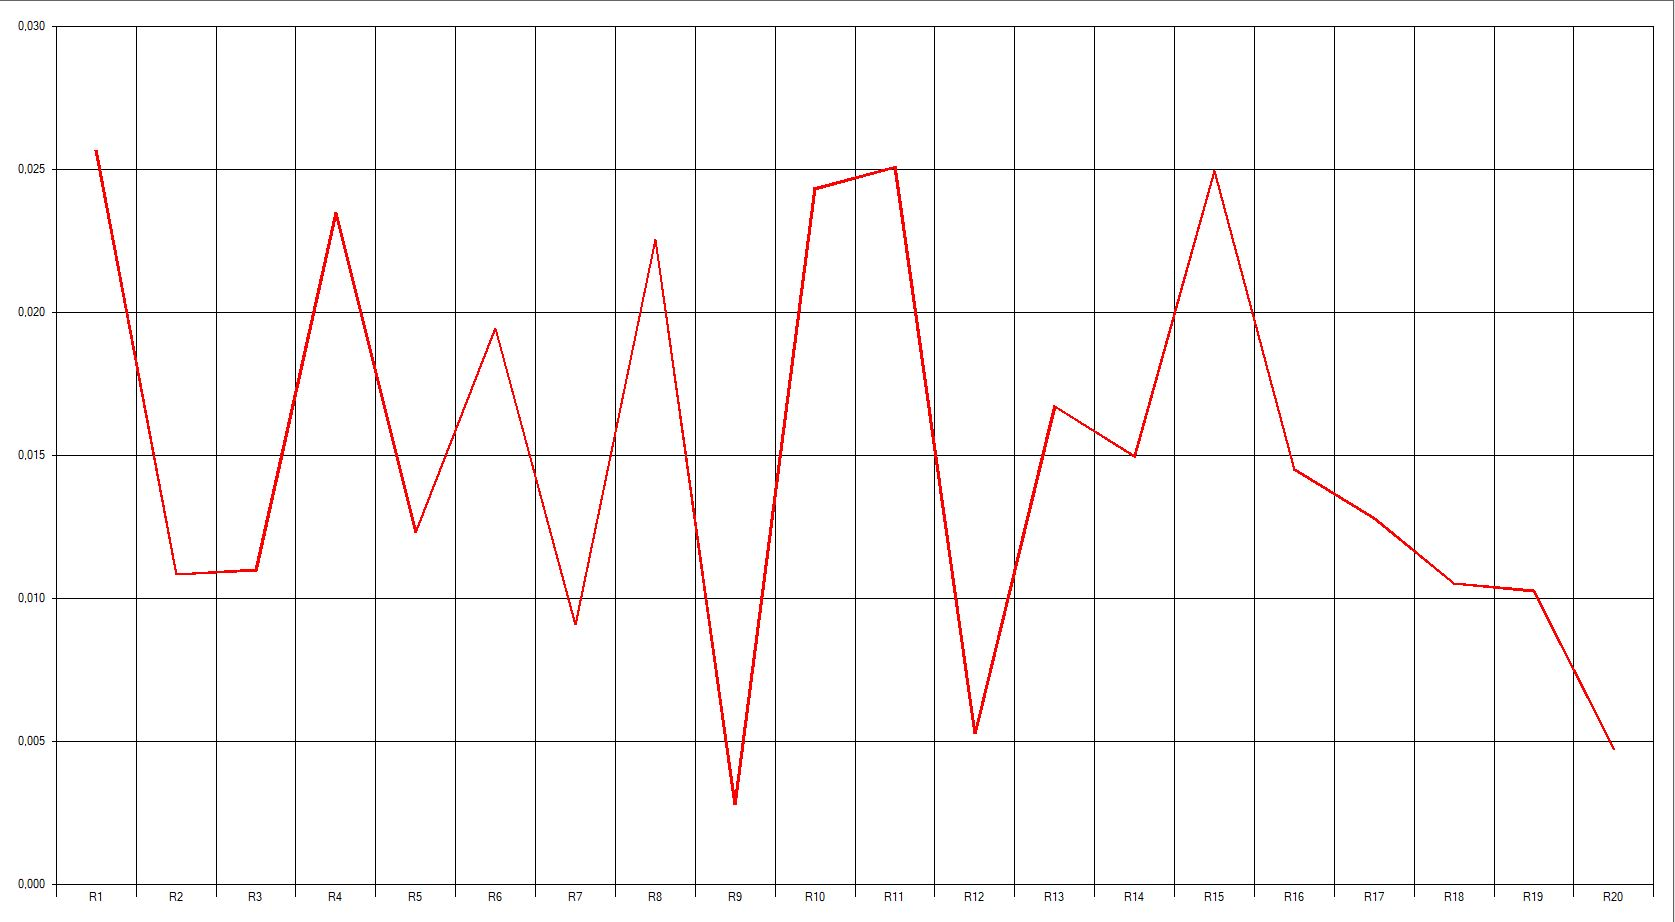
\includegraphics[width=0.8\textwidth]{Images/Photos/ErrorOP2.JPG} 
    \caption{Error progression without pruning for test} 
    \label{fig:ErrorOP2} 
\end{figure}

\begin{figure}[H] 
    \centering
    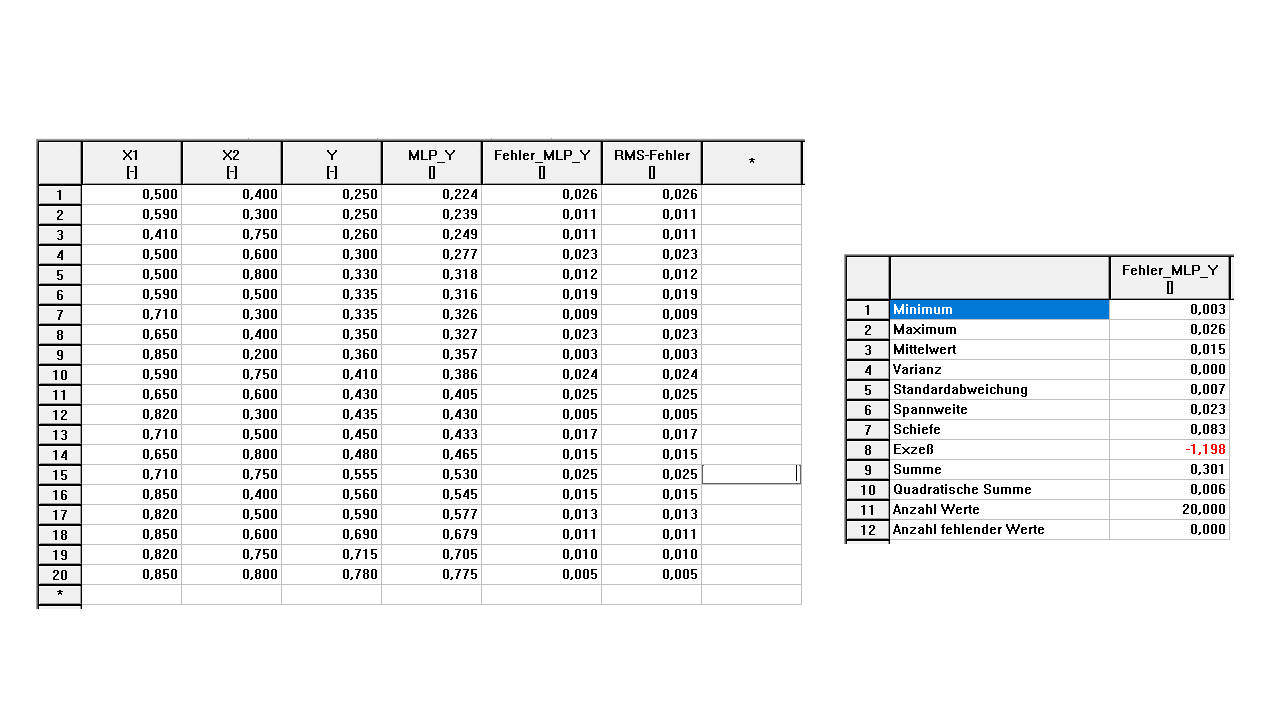
\includegraphics[width=0.9\textwidth]{Images/Fotos/Diapositiva12.PNG} 
    \caption{Results test} 
    \label{fig:ResultsTest} 
\end{figure}






%========================%
%        Math Models     %
%========================%

\newpage

\section{Mathematical models}

\par For the calculations, we will first define our Markov model, obtain the equations that will model the process and determine the connections between the elements that need to be made. To begin with, we will start from the idea that the model will have parallel active redundancy, which means that two components will be responsible for delivering the final result. As a consequence, instead of there being only two states, one of failure and the other of operation, now there are 4 for the combinations of the two components, because in case one fails, the other is still in operation. It is also going to be assumed that both components cannot fail at the same time.  Having said that, it is necessary to define some variables, as well as to clarify what is being assumed from the model.

\subsection{Calculations}

\par First, we begin by defining our inputs, outputs and ranges:
\begin{equation}
x_1 = \beta_1 \textit{; first stress parameter, which will be the enviromental temperature}
\end{equation}
\begin{equation}
x_2 = \beta_2 \textit{; second stress parameter, which will be the moisture or humidity in the enviroment}
\end{equation}
\begin{equation}
y = f \textit{; Output of the system}
\end{equation}

\par Also it is important to mention that according to the Markov model, it is assumed that $\tilde{\lambda}$ can be calculated through the following equation.

\begin{equation}
\tilde{\lambda}(t) = \lambda_0 + \lambda f(t)
\label{eq:Lambda}
\end{equation}
$$\lambda_0 = 0.04 \frac{1}{Tu}$$
$$\lambda = 0.05\frac{1}{Tu}$$
$$ f(t) =Y= \textit{output of the model} $$

\par Which states that if the value of $\lambda$ is above $0.05$ then the system will be under a bigger stress than usual. Therefore, its life time could be seen shorten

\par Once established the variables above, now it is time to develop the Markov model under the desired specifications of an active redundant model.

\par The number of states is going to be 4, since there are two components A and B, which could be on either one of two states, failure or operation.

$$\textit{State1} = P_1 (t)= (A,B)$$
$$\textit{State2} = P_2 (t)= (\overline{A} ,B)$$
$$\textit{State3} = P_3 (t)= (A,\overline{B})$$
$$\textit{State4} = P_4 (t)= (\overline{A},\overline{B})$$

\begin{figure}[H] 
    \centering
    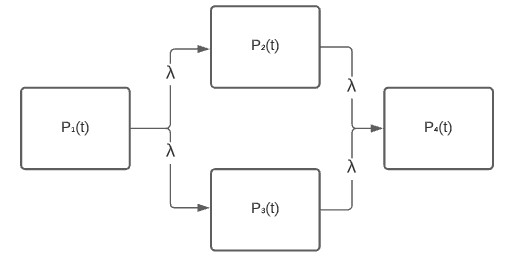
\includegraphics[width=0.5\textwidth]{Images/MarkovDiagram.JPG} 
    \caption{Model diagram} 
    \label{fig:ModelDiagram} 
\end{figure}

\par From the information above we can obtain the matrix for the model:

\begin{equation}
\begin{bmatrix}
\dot{P_1 (t)}\\
\dot{P_2 (t)}\\
\dot{P_3 (t)}\\
\dot{P_4 (t)}
\end{bmatrix}
= 
\begin{bmatrix}
-2\lambda & 0 & 0 & 0\\
 \lambda & -\lambda & 0 & 0\\
 \lambda & 0 & -\lambda & 0\\
 0 & \lambda & \lambda & 0
\end{bmatrix}
\begin{bmatrix}
P_1 (t)\\
P_2 (t)\\
P_3 (t)\\
P_4 (t)
\end{bmatrix}
\end{equation}

\par If we calculate the eigenvalues of the matrix, then we will also obtain that the system is stable,since there is just one value equal to zero, and the rest are lower than zero. And, as there are no conjugated roots, it will have an aperiodic behavior. 

\begin{equation}
\alpha = 
\begin{bmatrix}
\ 0 \\
\ - \lambda \\
\ - \lambda \\
\ -2 \lambda
\end{bmatrix}
\end{equation}

\par One last data that can be obtained from the matrix is the recommended simulation step. Since it is a matrix $4x4$, then the value of $n = 4$, while the maximum value of the matrix being $|a_{max}| = 2 \lambda$. This will give us that the step value must be of:

\begin{equation}
\Delta t< \frac{1}{4 (2 \lambda)} = \frac{1}{8 \lambda}
\end{equation}


\par Then, by analyzing each variable individually, we can get a set of differential equations:

$$ \frac{1}{2 \lambda} \dot{P_1 (t)} + P_1 (t) = 0 $$
$$ \frac{1}{\lambda} \dot{P_2 (t)} + P_2 (t) = P_1 (t) $$
$$ \frac{1}{\lambda} \dot{P_3 (t)} + P_3 (t) = P_1 (t) $$
$$ \dot{P_4 (t)} = \lambda [P_2 (t) + P_3 (t)]$$

\par The next step involves transforming into the Laplace domain the set of obtained differential equation, so they can be represented as transfer functions in the simulator.

$$ \frac{1}{2 \lambda} s P_1 (s) + P_1 (s) = ø $$
$$ \frac{1}{\lambda} s P_2 (s) + P_2 (s) = P_1 (s) $$
$$ \frac{1}{\lambda} s P_3 (s) + P_3 (s) = P_1 (s) $$
$$ s P_4 (s) = \lambda [P_2 (s) + P_3 (s)]$$

\vspace{10mm}
\begin{equation}
\frac{P_1 (s)}{ø} = \frac{1}{\frac{1}{2 \lambda} s + 1}
\label{eq: StateProbability}
\end{equation}
$$ \frac{P_2 (s)}{P_1 (s)} = \frac{1}{\frac{1}{\lambda} s + 1}$$
$$ \frac{P_3(s)}{P_1 (s)} = \frac{1}{\frac{1}{\lambda} s + 1}$$
$$ \frac{P_4 (s)}{P_2 (s) + P_3 (s)} = \frac{\lambda}{s}$$

\par Finally, with this information we are now able to represent the model in any simulator. In our case, DynStar is going to be used.

\par One last point to remark is that, for the hybrid Markov model, instead of calculating $\lambda$ as a constant, it is going to be directly used the output of \ref{eq:Lambda}, meaning that this value is going to be always dynamic.

\subsection{Expected results}

\par With all this information, parameters, variables and conditions, it is now possible to represent the calculations and model in the simulator.

\begin{figure}[H] 
    \centering
    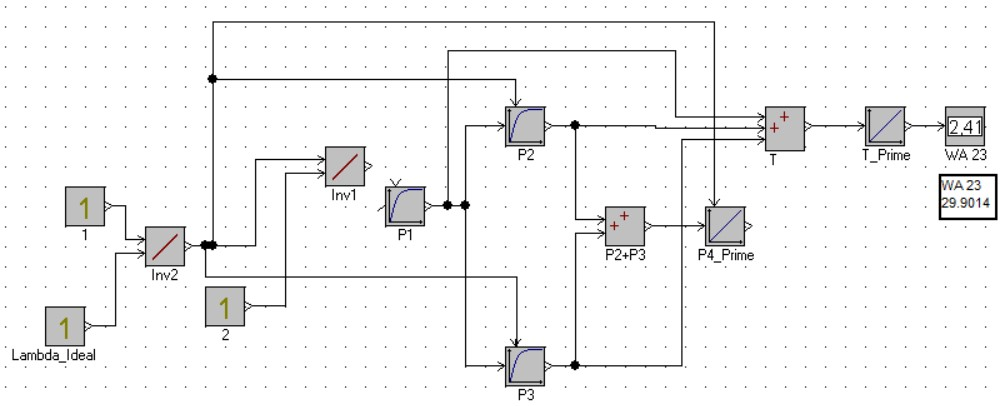
\includegraphics[width=0.8\textwidth]{Images/ConnectionsIdeal.JPG} 
    \caption{Ideal model diagram} 
    \label{fig:IdealDiagram} 
\end{figure}

\par As it can be seen, the result is very near to 30 time units. By applying Equation \ref{eq:T2} with the value of ${\lambda} = 0.05$ it is clear that the implementation of the model is correct, and that the value should be 30. The reason behind the difference between the pure calculations and the simulation is the same simulation, as due to the numeric methods used by the software, there is a certain error.

\begin{figure}[H] 
    \centering
    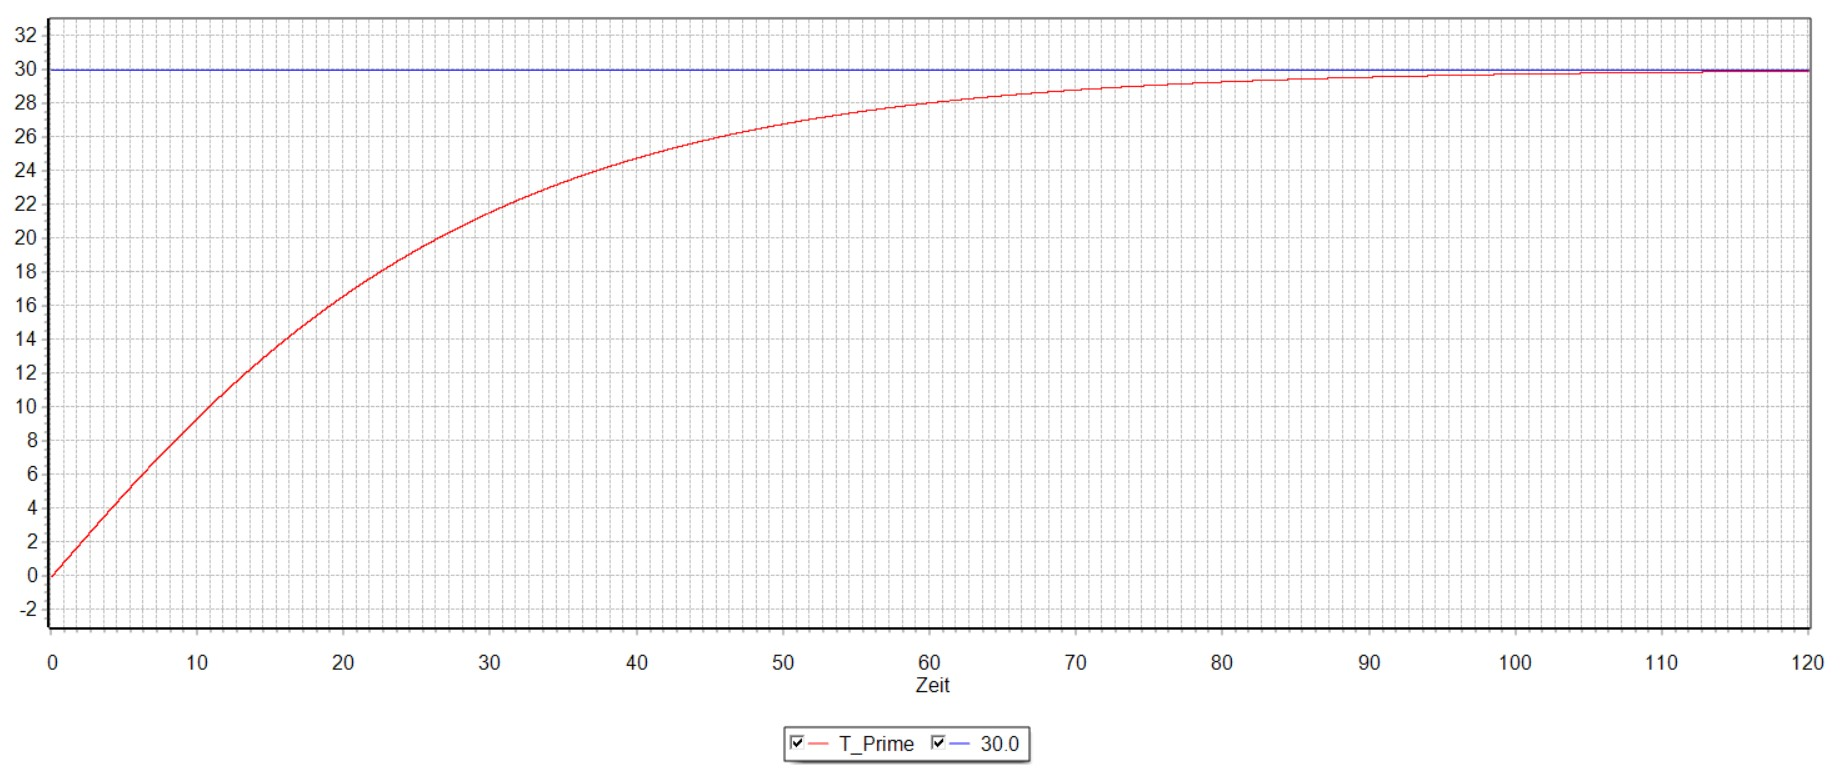
\includegraphics[width=0.95\textwidth]{Images/TimeLifeIdeal.JPG} 
    \caption{Ideal time life} 
    \label{fig:IdealT} 
\end{figure}

\par Another important aspect or behavior that should be also seen on the final model is that the sum of the states must always be equal to 1 or 100\%, and the intersection between the probabilities of the 4 states must be near to 13.8 units of time.

\begin{figure}[H] 
    \centering
    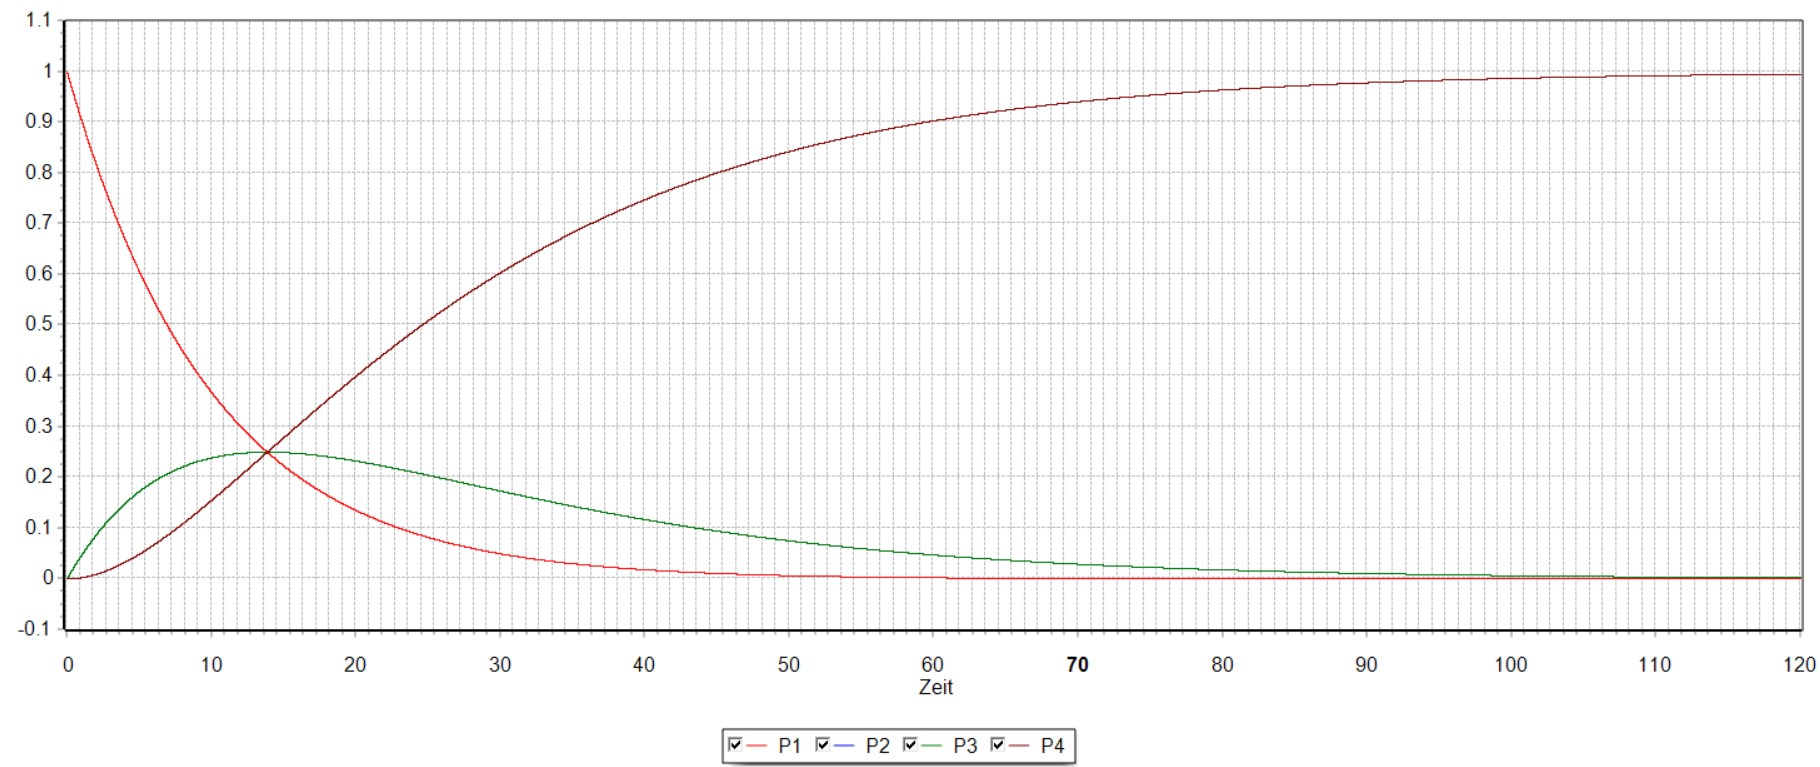
\includegraphics[width=0.95\textwidth]{Images/StatesIdeal.JPG} 
    \caption{Ideal rates} 
    \label{fig:IdealRates} 
\end{figure}

\par The last aspect to consider is that, as well as in the previous graph, the failure and survival rates will complement each other, and that the intersection of these two will happen around 24.56 units of time, and the time life will come when the failure rate is at about 60\%, as in Figure \ref{fig:IDTL}.

\begin{figure}[H] 
    \centering
    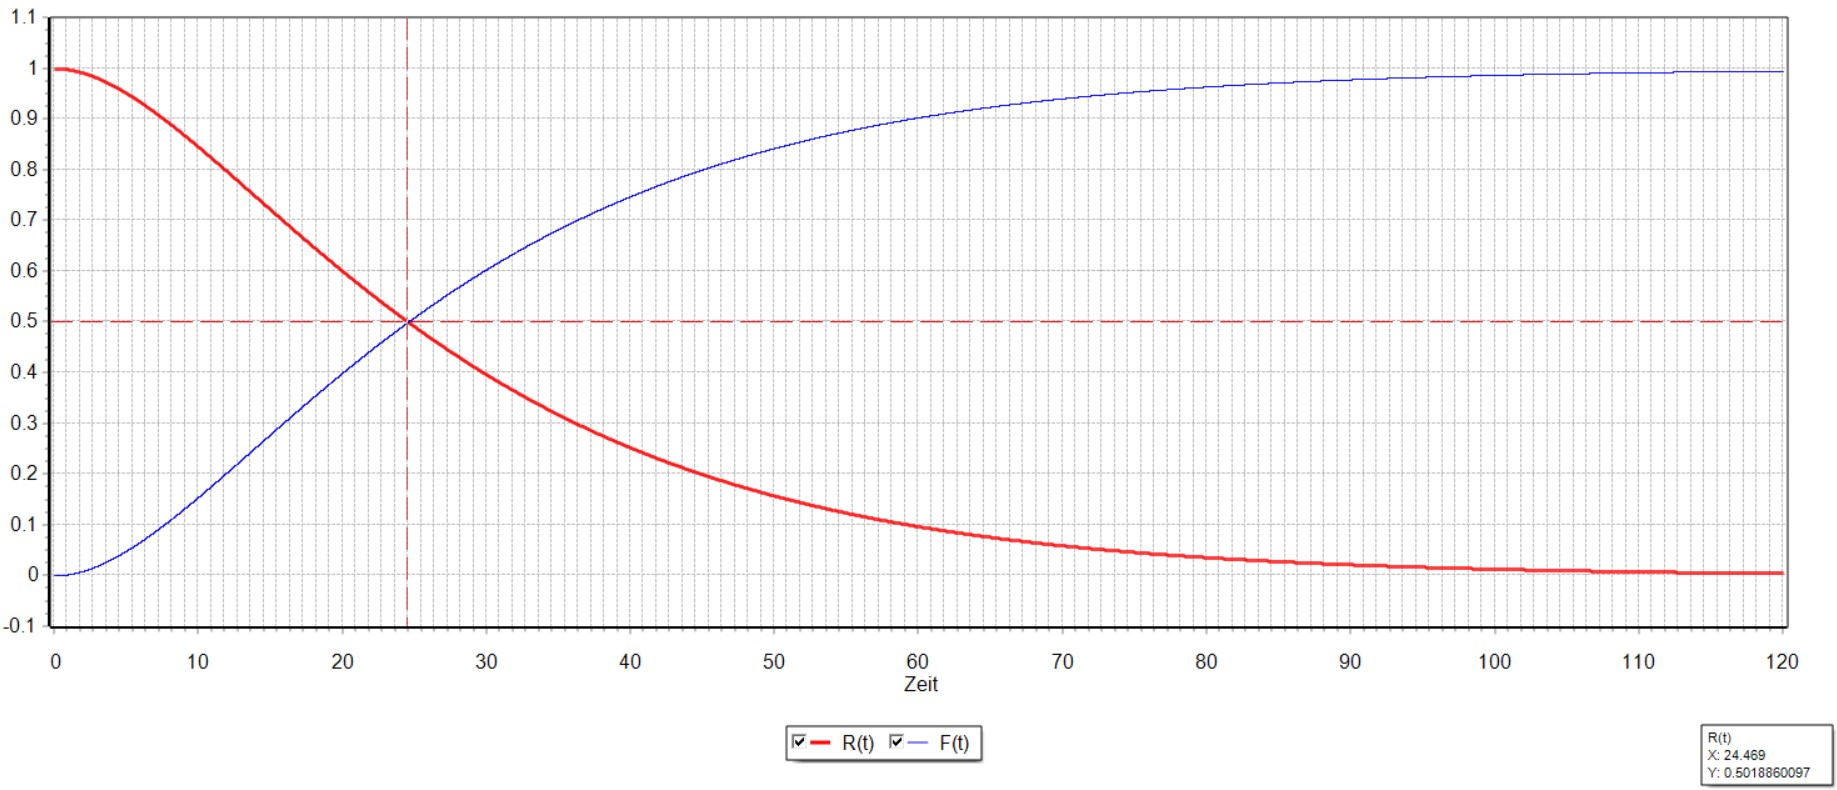
\includegraphics[width=0.95\textwidth]{Images/FSIdIn.JPG} 
    \caption{Intersection between failure and survival rates } 
    \label{fig:IDIN} 
\end{figure}

\begin{figure}[H] 
    \centering
    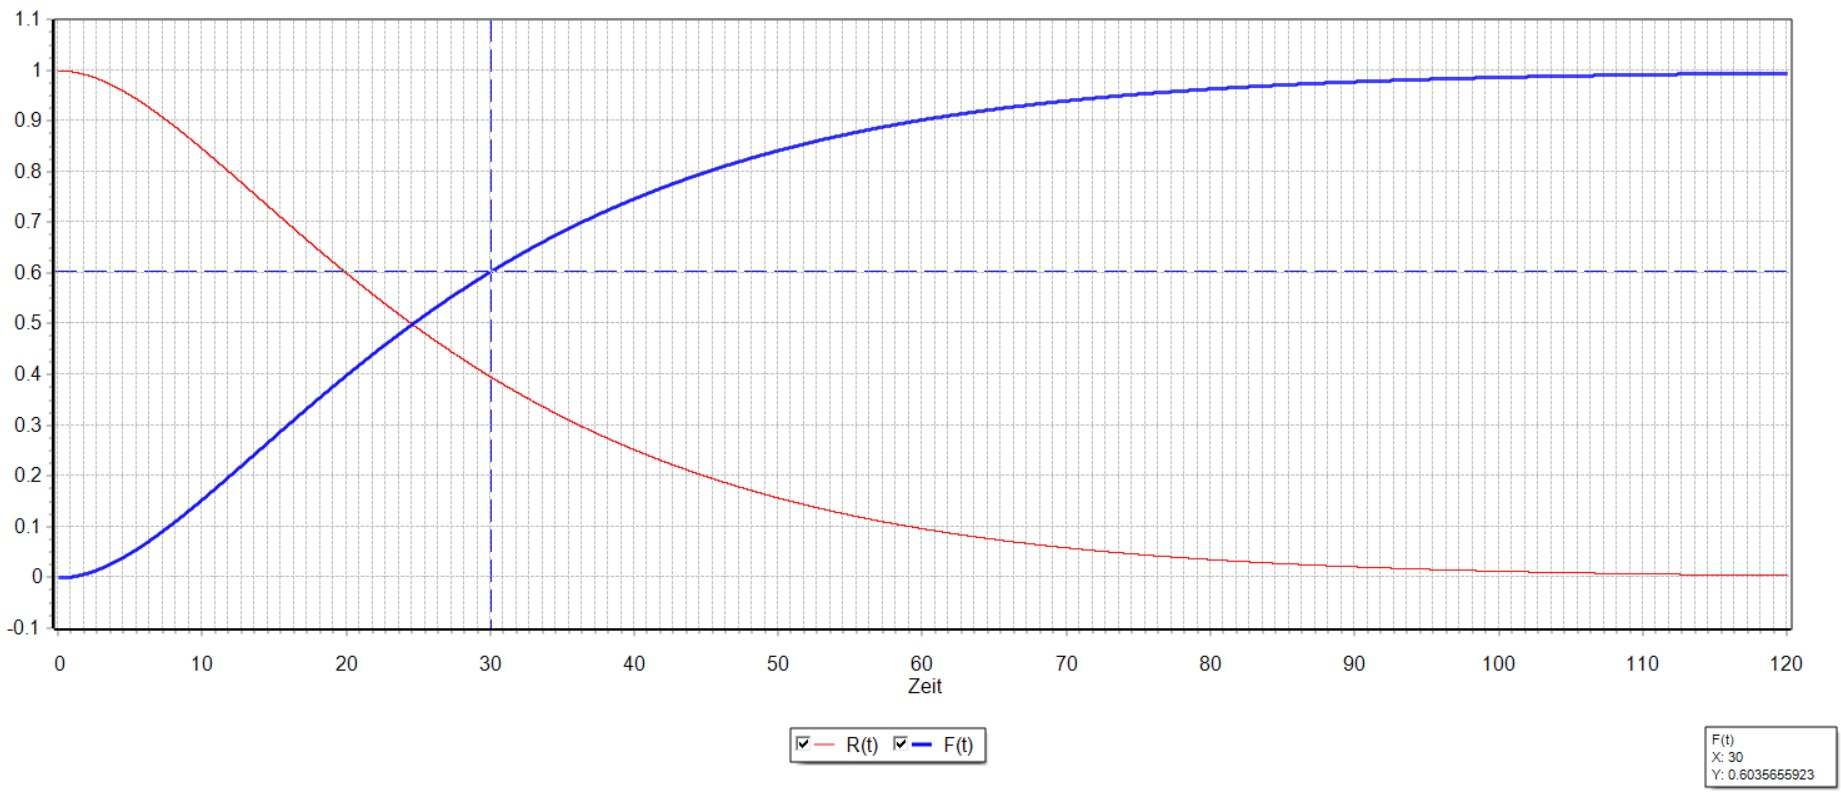
\includegraphics[width=0.95\textwidth]{Images/FSIdTL.JPG} 
    \caption{Failure probability at the obtained lifetime} 
    \label{fig:IDTL} 
\end{figure}

\par One last thing, returning to the mathematical model, the system matrix will look as follows:

\begin{equation}
\begin{bmatrix}
\dot{P_1 (t)}\\
\dot{P_2 (t)}\\
\dot{P_3 (t)}\\
\dot{P_4 (t)}
\end{bmatrix}
= 
\begin{bmatrix}
-2(0.05) & 0 & 0 & 0\\
 (0.05) & -(0.05) & 0 & 0\\
 (0.05) & 0 & -(0.05)& 0\\
 0 & (0.05)bs & (0.05) & 0
\end{bmatrix}
\begin{bmatrix}
P_1 (t)\\
P_2 (t)\\
P_3 (t)\\
P_4 (t)
\end{bmatrix}
\end{equation}

\par with its eigenvalues being:

\begin{equation}
\alpha = 
\begin{bmatrix}
\ 0 \\
\ - (0.05) \\
\ - (0.05) \\
\ - (0.1)
\end{bmatrix}
\end{equation}

\par And the suggested simulation step size being of:

\begin{equation}
\Delta t< \frac{1}{4 (2 (0.05))} = \frac{1}{0.4}=2.5 TU
\end{equation}


%========================%
%         Simulation     %
%========================%

\newpage

\section{Simulation models}

\par Once the theoretical framework, the calculations, the MLP model and the transfer functions of all the components are complete. Now we proceed to make the relevant connections. As can be seen in Figure \ref{fig:ModelDiagram}, this is the configuration to be followed for the redundant active Markov model, in this configuration the transfer functions calculated in the previous step will be added and the connections will be made.

\subsection{Simulation parameters}

\par Regarding the requirements for the simulation, first of all it is necessary to define the simulation time, which will be 120 TU and the step of each pulse, this being 0.01 TU, just because practical experience tell us that it should give a precise result. The next task on the list is to define the stress conditions or the values of the inputs that will help us to determine the system lifetime. In Figures \ref{fig:InputGraph} and \ref{fig:InputTable} we can see both inputs defined as a table and graphically. The first input or $ X_1 = \beta_1$ will stand for the temperature, while the second input  $ X_2 = \beta_2$ will stand for the humidity or moisture of the environment; therefore, they both stand for the changing of environmental conditions.

\begin{figure}[H] 
    \centering
    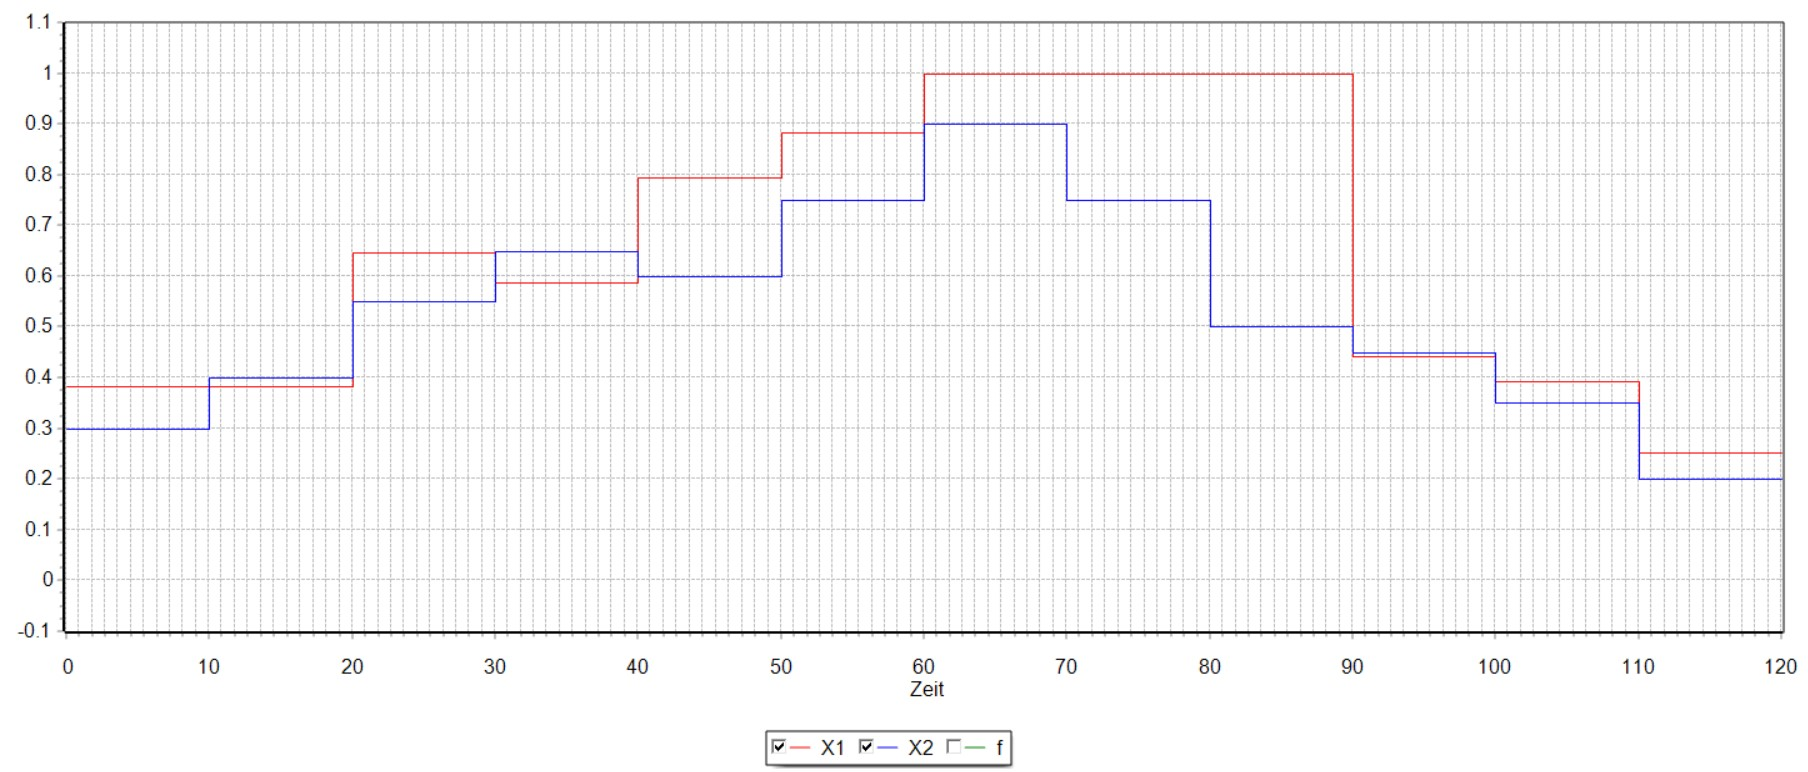
\includegraphics[width=1.0\textwidth]{Images/InputGraph.JPG} 
    \caption{Input graph} 
    \label{fig:InputGraph} 
\end{figure}

\begin{figure}H] 
    \centering
    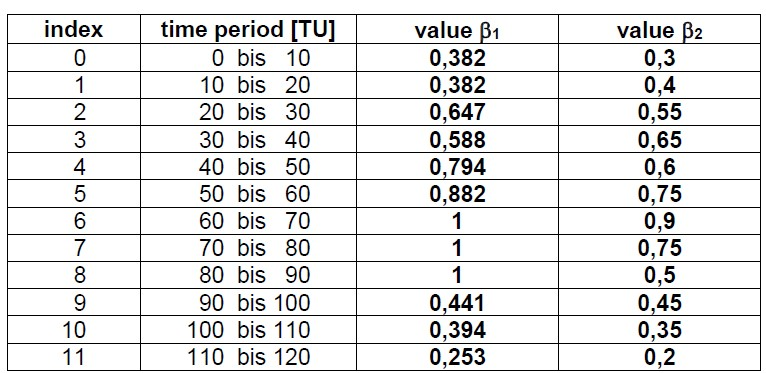
\includegraphics[width=0.7\textwidth]{Images/InputTable.JPG} 
    \caption{Input table} 
    \label{fig:InputTable} 
\end{figure}


\vspace{10mm}

\subsection{Connections}

\par The connections are quite simple as for Equation \ref{eq:Lambda} this is represented by Figure \ref{fig:SimulationEquation}, in which an integrator was also added, which helps to calculate the average value together with the value of the elapsed time, configured as a divisor of the integral result. The result of this scheme will allow us to calculate $\tilde{\lambda}$, which will give us a general idea of the stress conditions.

\begin{figure}[H] 
    \centering
    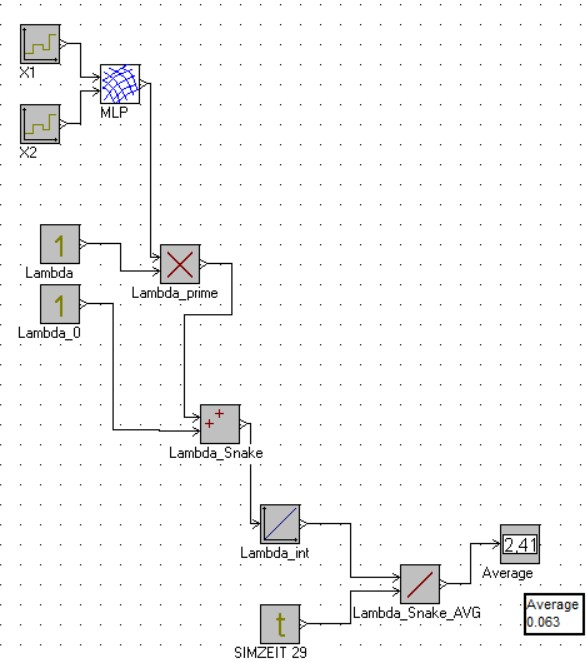
\includegraphics[width=0.4\textwidth]{Images/SimulationEquation.JPG} 
    \caption{Simulation of the $\lambda$ equation: scheme} 
    \label{fig:SimulationEquation} 
\end{figure}

\par The following section is merely the configuration of Figure \ref{fig:ModelDiagram} in the simulator. As can be seen in Figure \ref{fig:SimulationModel}, blocks of transfer functions are used to represent the different states. There is no input per se, but the system itself must tend towards a behavior. What is seen in the connections is the value of $\tilde{\lambda} $ applying to each block. 

\begin{figure}[H] 
    \centering
    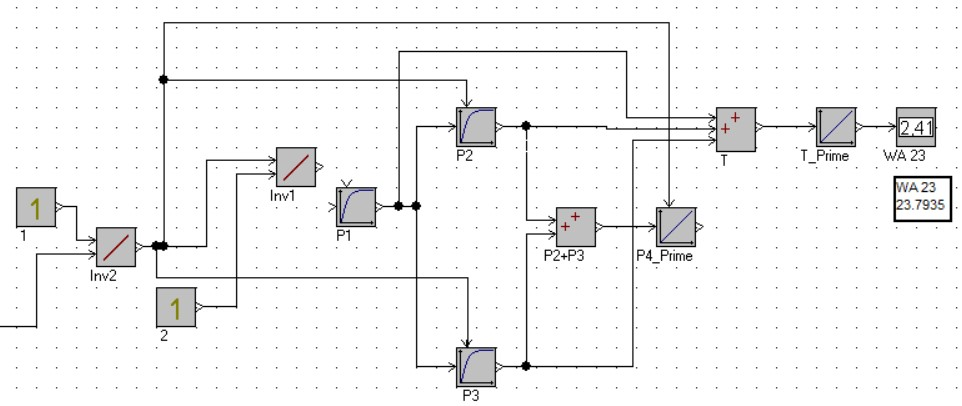
\includegraphics[width=0.7\textwidth]{Images/SimulationModel.JPG} 
    \caption{Simulation of the state model: scheme} 
    \label{fig:SimulationModel} 
\end{figure}


\subsection{Comparison}

\par The major differences between the classical Markov model and the hybrid model come from the origin of $\lambda$, since in the case of the classical model, $\\lambda$ is a constant variable, which, is already given by the mathematical model and this is $\lambda = 0.05$. However, in the hybrid model, the life time calculation is improved by the use of a dynamic $\lambda$, which should, in principle, be much closer to reality.


\subsubsection{Classical Markov model}

\begin{figure}[H] 
    \centering
    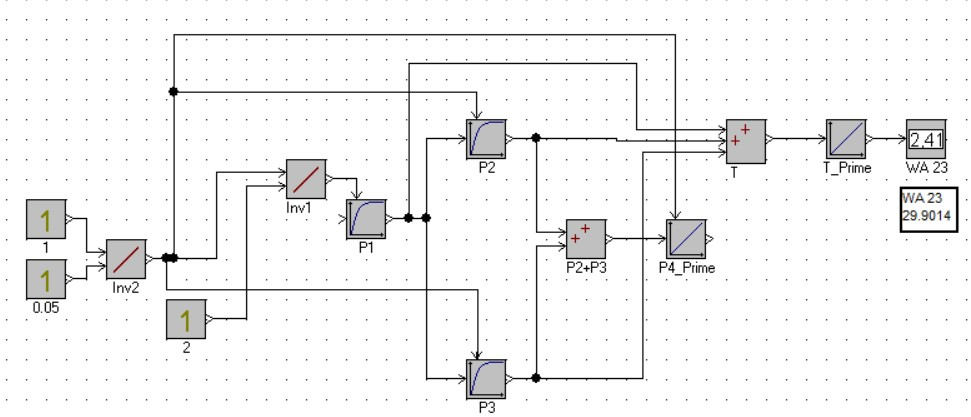
\includegraphics[width=0.9\textwidth]{Images/ClassicalModel.JPG} 
    \caption{Classical Markov model: scheme} 
    \label{fig:ClassicalModel} 
\end{figure}

\par As for the classical model, $\lambda$ is directly applied as a constant to the other blocks of the states. 



\subsubsection{Hybrid Markov model}

\begin{figure}[H] 
    \centering
    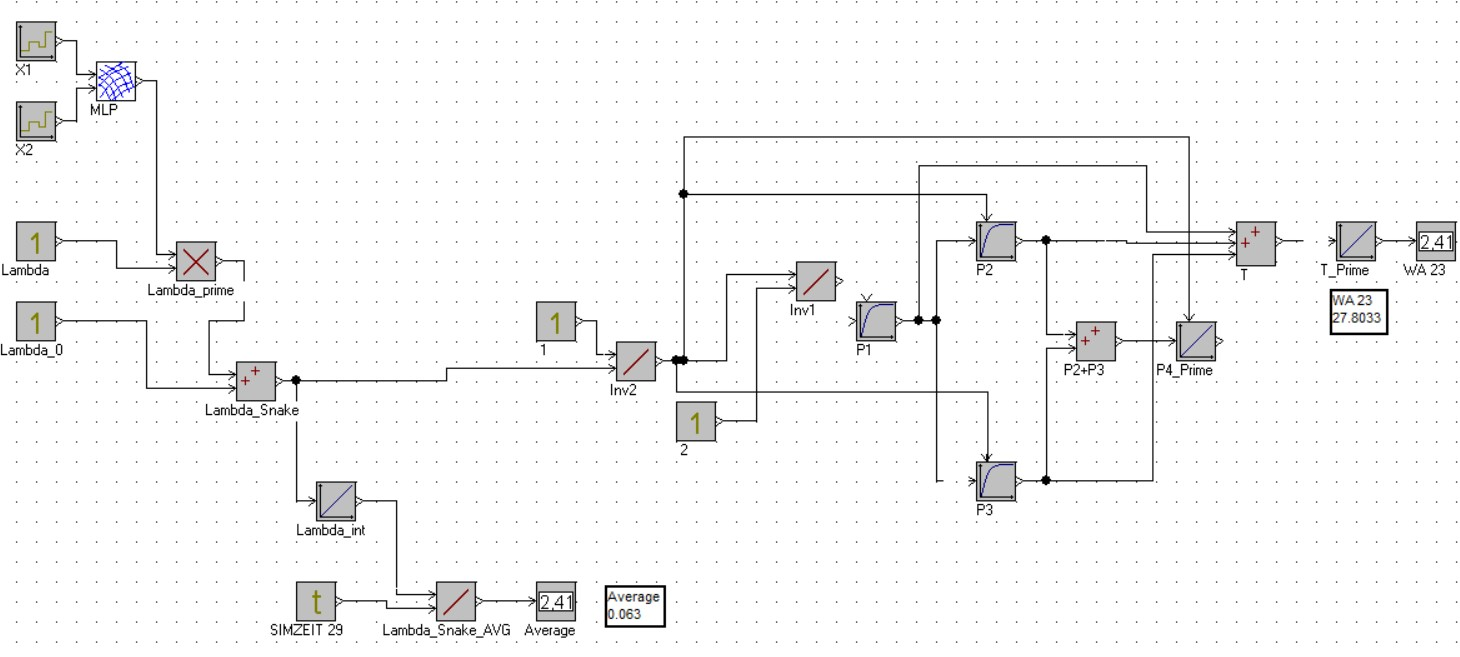
\includegraphics[width=0.9\textwidth]{Images/HybridModel.JPG} 
    \caption{Hybrid Markov model: scheme} 
    \label{fig:HybridModel} 
\end{figure}

\par While for the hybrid model, the raw value of $\lambda$ from the MLP value and the mathematical model is directly applied to the state blocks to perform the calculations. 






%========================%
%          Results       %
%========================%
\newpage

\section{Simulation results}

\par As for the results, 5 graphs will be obtained from the simulation. The first one describes the behavior of the stress conditions or inputs as well as the output from the MLP model. A second one with the $\lambda$ value together with the average $\tilde{\lambda}$, and the ideal $\lambda$ of $0.05$ . These two should be the same for both the classical and hybrid models. Subsequently, the third plot is of the probability that the model is in one of the four states. In this graph, the most relevant value is the intersection of all the states, since the effects of lifetime can be reflected in this value. The fourth graph represents the lifetime of the model and therefore of the system being modeled. And the fifth represents the failure and survival rates together.

\subsection{Raw results}

\par As for the results of the first plot in Figure \ref{fig:MLPOutput}, there is not much to say, it is simply how the model would react to the stress conditions introduced. It should be emphasized that the results meet the expectations of range between [0,1], so there is no error or strange situation that jumps out at first sight.

\begin{figure}[H] 
    \centering
    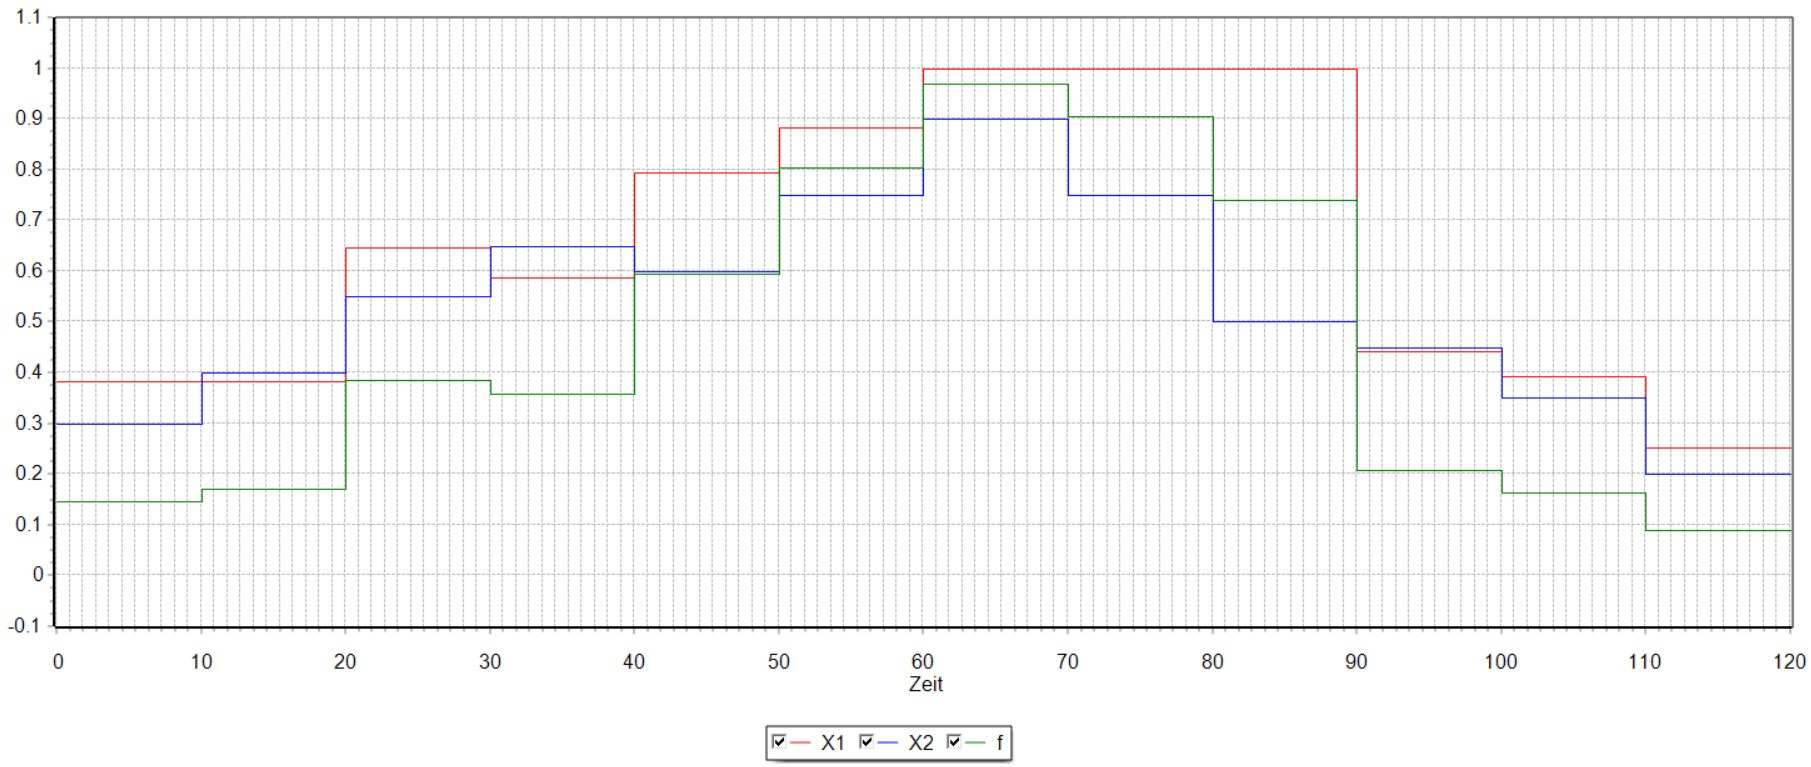
\includegraphics[width=1.0\textwidth]{Images/MLPOutput.JPG} 
    \caption{Stress conditions and MLP output graph} 
    \label{fig:MLPOutput} 
\end{figure}

\par For the second plot in Figure \ref{fig:LambdaCalculation}, average $\tilde{\lambda}$ divides the $\lambda$ output into two parts, where, precisely because of the $\lambda$ values above the average $\tilde{\lambda}$ value, this last variable rises above the ideal value of 0.05, which in turn, mathematically reduces the lifetime.

\begin{figure}[H] 
    \centering
    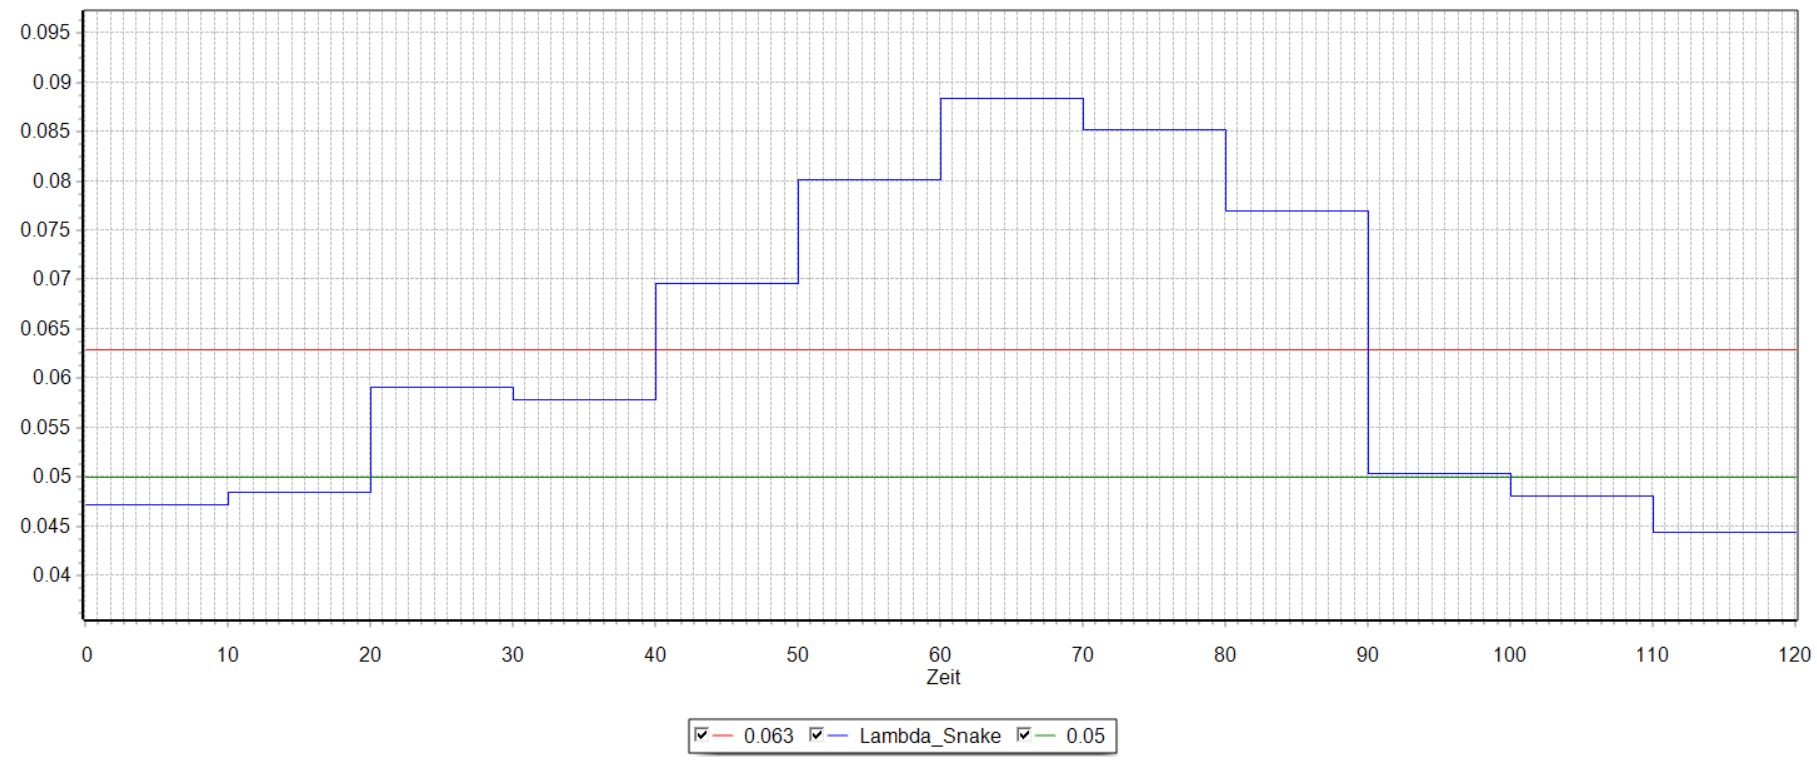
\includegraphics[width=1.0\textwidth]{Images/LambdaCalculation.JPG} 
    \caption{$\tilde{\lambda}$ calculation} 
    \label{fig:LambdaCalculation} 
\end{figure}



\subsection{Comparison}

\par As already mentioned, the main points of interest will be the point of intersection in the third plot between the probability of the four states, since depending on where this is, the lifetime of the model can be approximated for constant $\lambda$. Another point to take into account, of course, will be the value of the lifetime of the simulations because with them the differences between one model and the other will be directly seen.

\subsubsection{Classical Markov model}

\par In the classical model, the intersection of the probabilities of the 4 states occurs around 13.8 time units, a situation that is reflected in the fourth graph, which has a lifetime of around 30 time units.

\begin{figure}[H] 
    \centering
    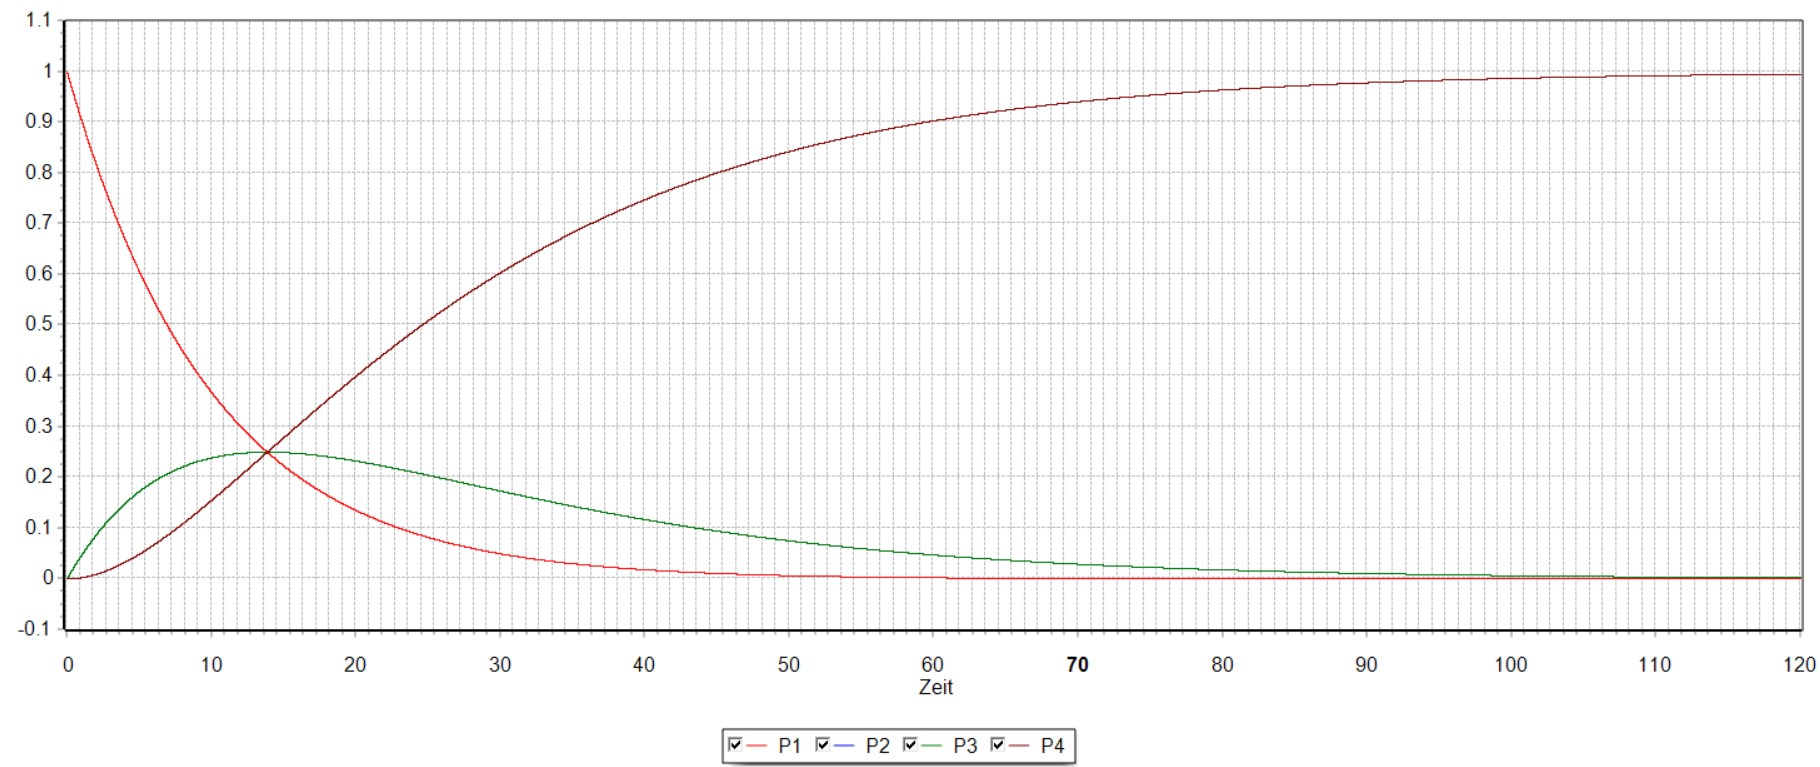
\includegraphics[width=0.75\textwidth]{Images/StatesIdeal.JPG} 
    \caption{Classical Markov model: states probabilities} 
    \label{fig:HybridStatesC} 
\end{figure}

\begin{figure}[H] 
    \centering
    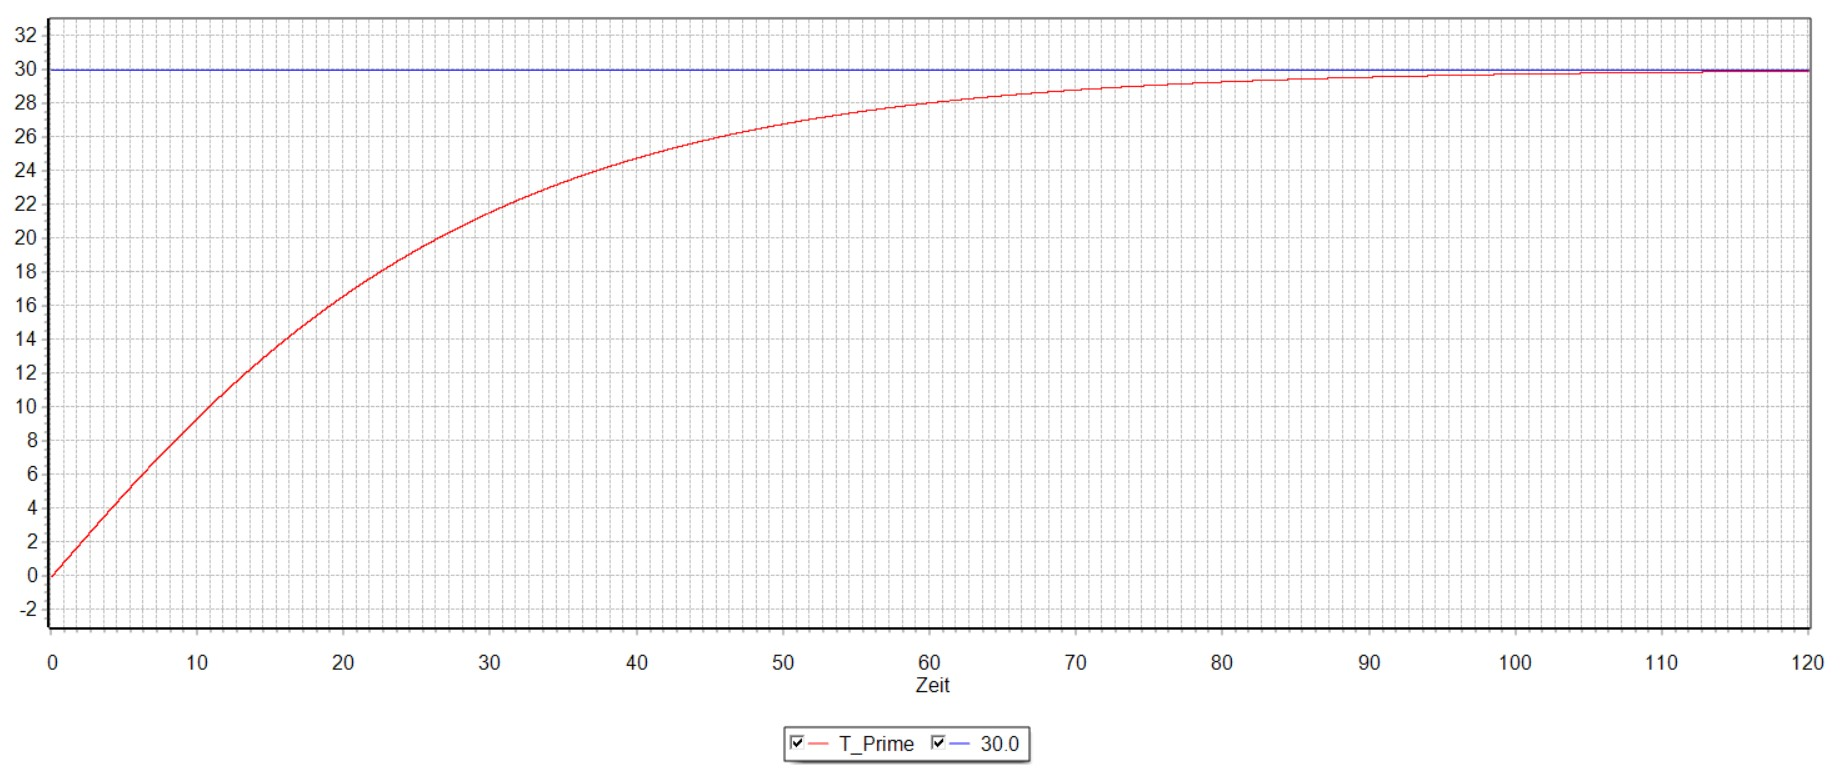
\includegraphics[width=0.75\textwidth]{Images/TimeLifeIdeal.JPG} 
    \caption{Classical Markov model: lifetime } 
    \label{fig:HybridTimeLifeC} 
\end{figure}


\par For the last graph, we get that the intersection between the failure and survival rates is about 24.56 units of time, while the obtained lifetime occurs when the failure probability is at about 57.5\%.

\begin{figure}[H] 
    \centering
    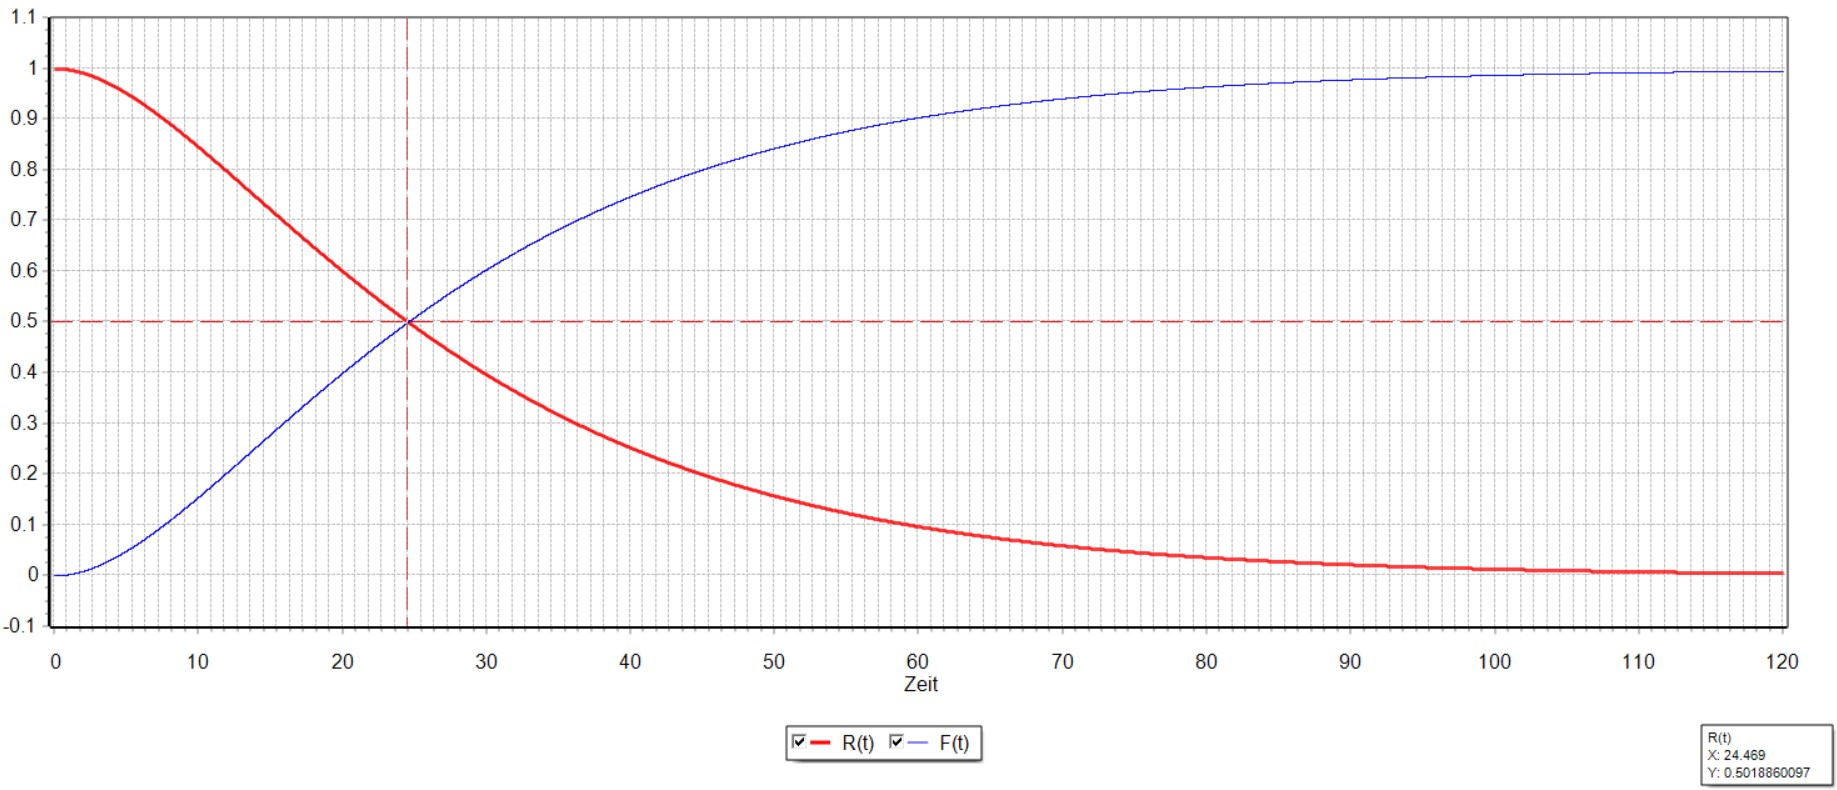
\includegraphics[width=0.75\textwidth]{Images/FSIdIn.JPG} 
    \caption{Classical Markov model: failure and survival rates} 
    \label{fig:FSCIn} 
\end{figure}

\begin{figure}[H] 
    \centering
    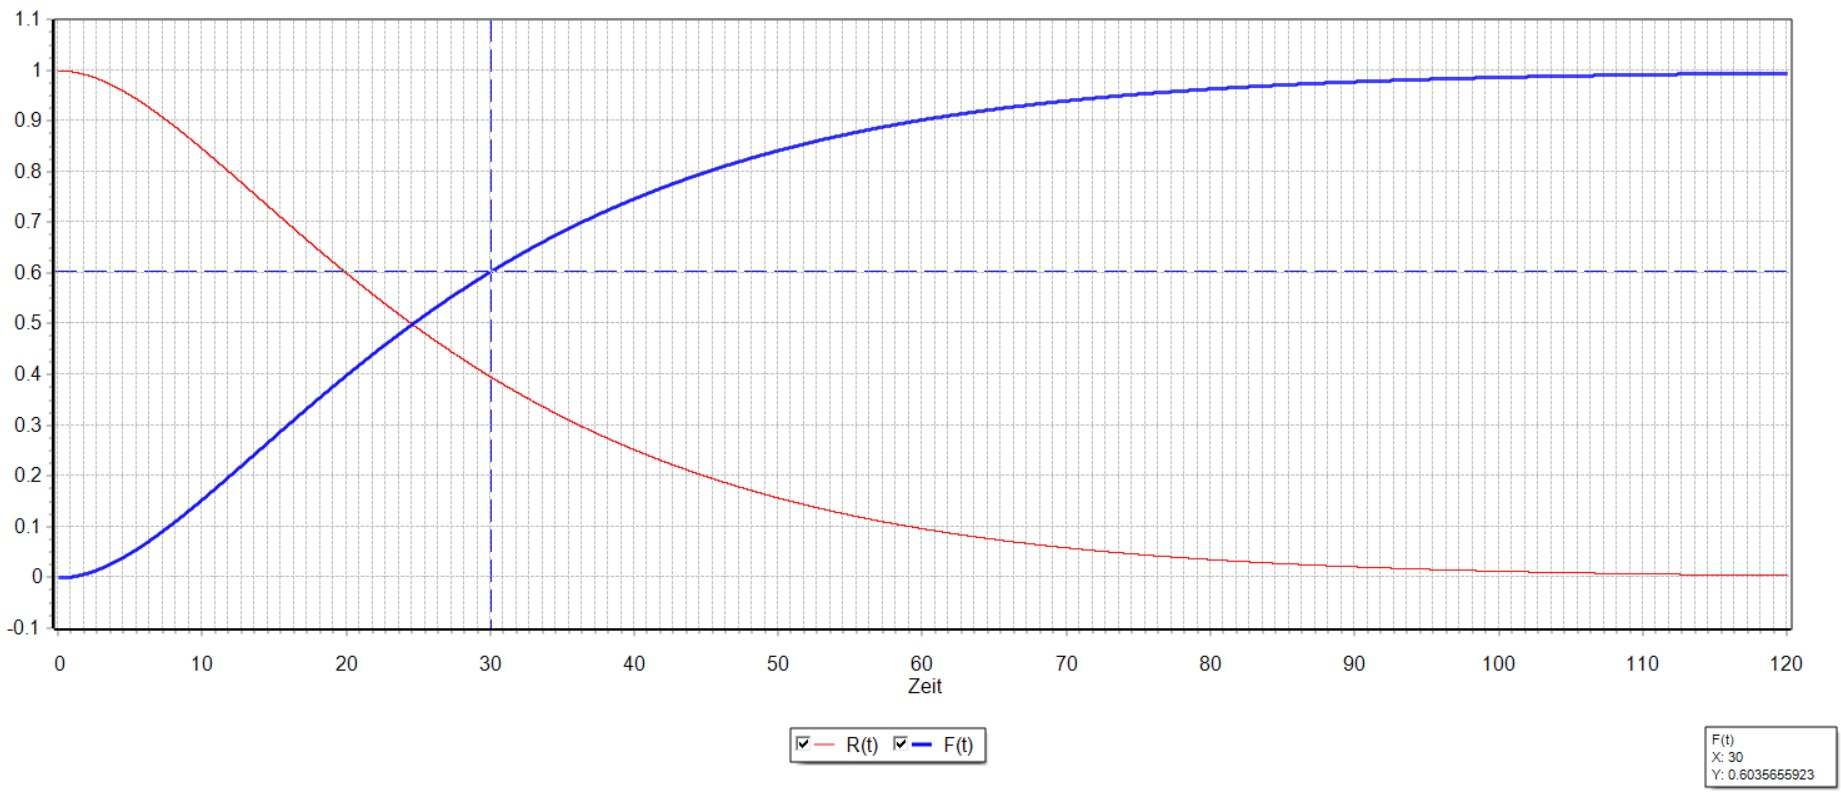
\includegraphics[width=0.75\textwidth]{Images/FSIdTL.JPG} 
    \caption{Classical Markov model:Failure rate at obtained lifetime} 
    \label{fig:FSCLT} 
\end{figure}



\subsubsection{Hybrid Markov model}

\par While in the classical model, the intersection of the probabilities of the 4 states is around 14.4 time units, which translates into 27.8 time units in the life time.

\begin{figure}[H] 
    \centering
    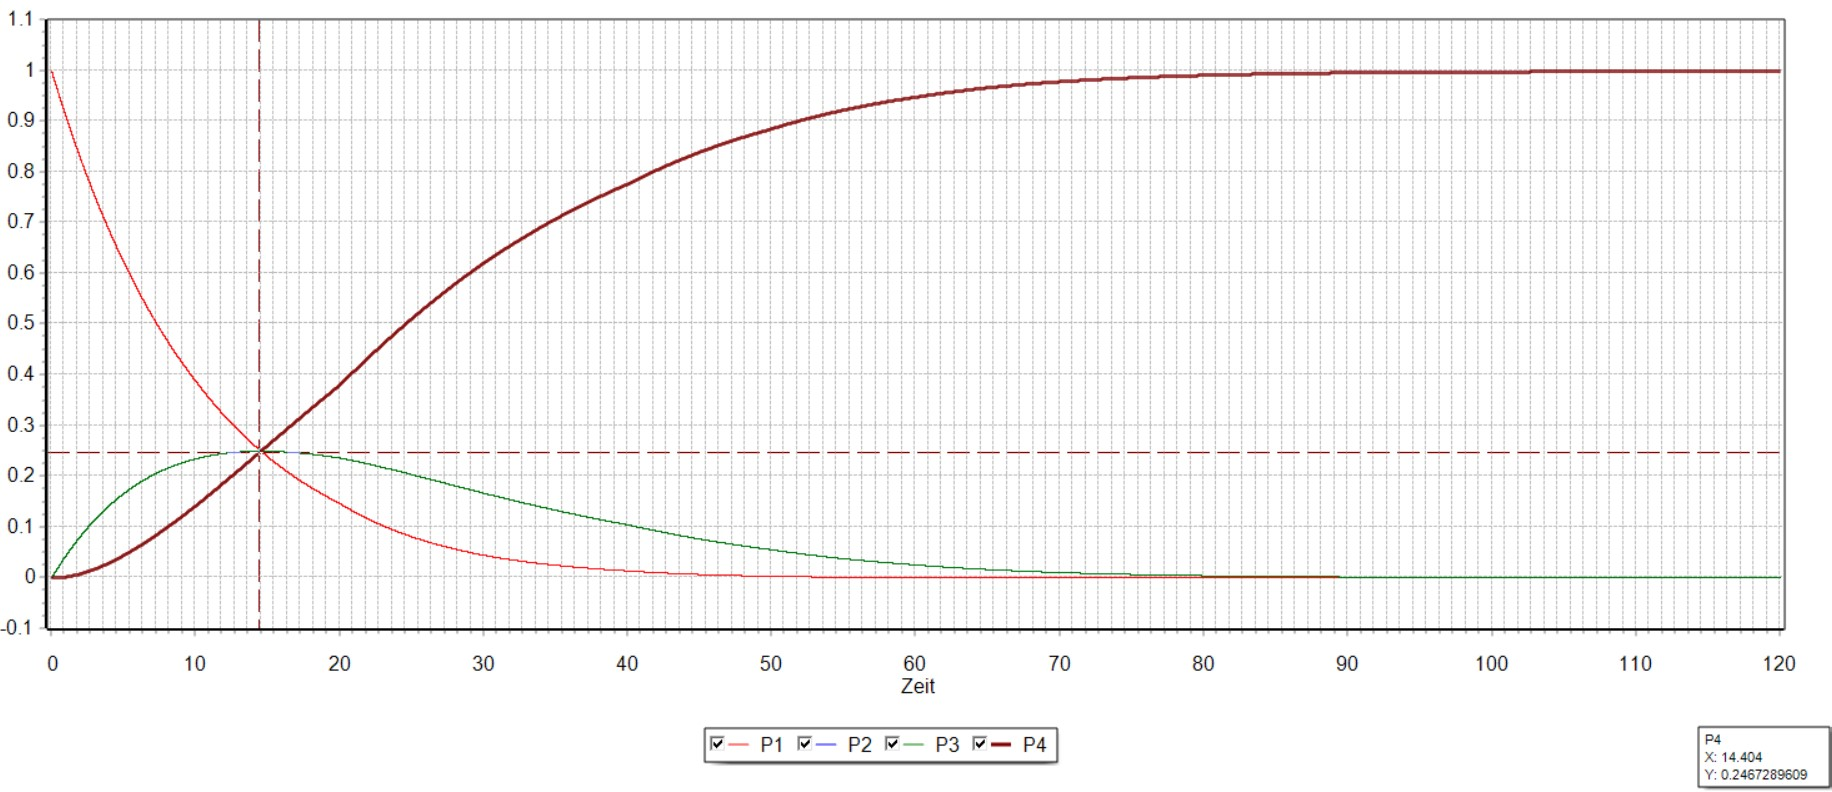
\includegraphics[width=0.75\textwidth]{Images/HybridStates.JPG} 
    \caption{Hybrid Markov model: states probabilities} 
    \label{fig:HybridStatesH} 
\end{figure}

\begin{figure}[H] 
    \centering
    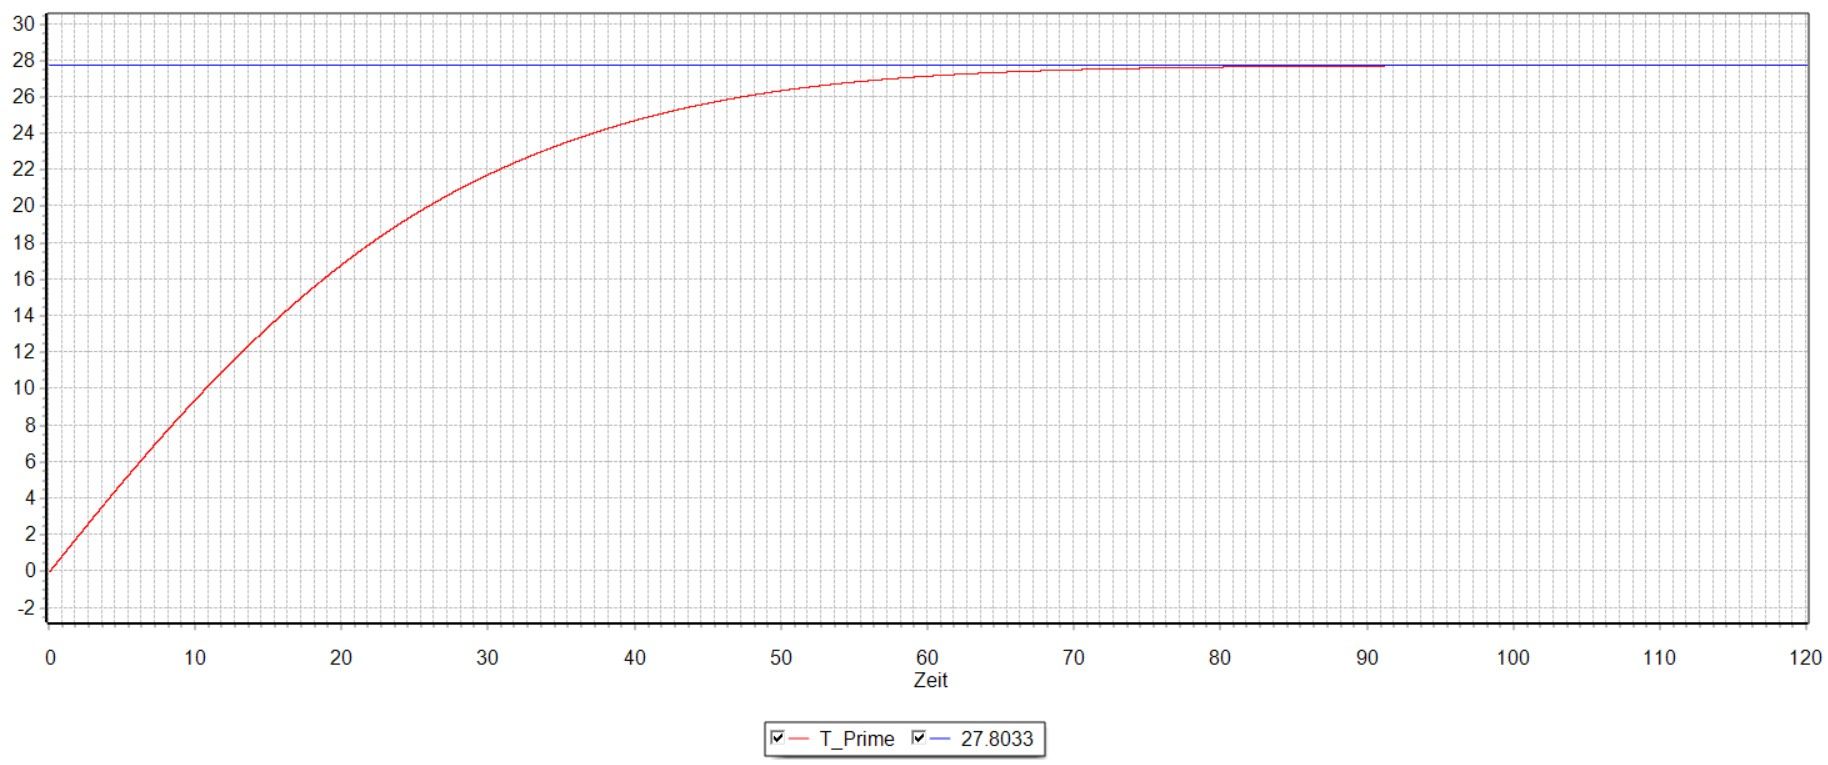
\includegraphics[width=0.75\textwidth]{Images/HybridTimeLife.JPG} 
    \caption{Hybrid Markov model: lifetime} 
    \label{fig:HybridTimeLifeH} 
\end{figure}

\par For the last graph, we get that the intersection between the failure and survival rates is now about 24.56 units of time, while the obtained lifetime occurs when the failure probability is at about 57.5\%. 

\begin{figure}[H] 
    \centering
    \includegraphics[width=0.75\textwidth]{Images/FSHIn.JPG} 
    \caption{Hybrid Markov model: lifetime failure and survival rates} 
    \label{fig:FSHIn} 
\end{figure}

\begin{figure}[H] 
    \centering
    \includegraphics[width=0.75\textwidth]{Images/FSHLT.JPG} 
    \caption{Hybrid Markov model: Failure rate at obtained lifetime} 
    \label{fig:FSHLT} 
\end{figure}






\newpage

\section{Evaluation}

\par Finally we come to the evaluation section. After having done the corresponding simulation of the states, it was obtained that the hybrid model results in a shorter lifetime than the classical model.However, the reasons behind these results, are not yet explained.

\subsection{Comparison}

\par Compared to the classical model the hybrid model shows a decrease in lifetime. This directly means that the stress conditions are quite demanding and, by placing more demands on the model, they detract from its lifetime. Mathematically, this can be understood by the only variable contributing to the changes in the system being $\tilde{\lambda}$. While in the classical model $\lambda$ is equal to 0.05, in the hybrid model the average of this value equals 0.063. In principle, the difference is not so large, but since it is an exponential distribution, small differences are amplified. The closer $\tilde{\lambda}$ is to that of the classical model, 0.05, the closer the result will resemble the theoretical results. Therefore, just with this value it can already be concluded that the system is under higher environmental conditions and will under-perform. 

\par For the direct comparison of the graphs, we can see in Figure \ref{fig:CSP} that the states probabilities is almost the same for both models; nonetheless, as it was already stated, the hybrid model takes a longer time to reach the 25\% for all states, which could indicate a higher life time, but this is not the case as seen in Figure \ref{fig:CLT}.
\begin{figure}[H] 
    \centering
    \includegraphics[width=0.75\textwidth]{Images/ComparisonStates.JPG} 
    \caption{Comparison between the states probabilities} 
    \label{fig:CSP} 
\end{figure}

\begin{figure}[H] 
    \centering
    \includegraphics[width=0.75\textwidth]{Images/ComparisonTL.JPG} 
    \caption{Life-time comparison} 
    \label{fig:CLT} 
\end{figure}

\par Visually, it can be seen in Figure \ref{fig:CFS}, as the intersection between the failure and survival rate occurs earlier with the hybrid model, meaning that the failure rate when the life-time occurs is also higher than in the classical model, and that the hybrid model presents a much quicker decay than the classical one.

\begin{figure}[H] 
    \centering
    \includegraphics[width=0.75\textwidth]{Images/ComparisonRates.JPG} 
    \caption{Failure and survival rates comparison} 
    \label{fig:CFS} 
\end{figure}

\par With all this information in can be deducted that even though the classical model presents a much more optimistic projection. The hybrid model  presents a much reserved prognosis, based on the actual stress conditions, and shows a more precise model of reality.

\subsubsection{Dynamics: Classical Markov model}

\par On the part of the classical model, the value of $\lambda$ does not undergo changes and the exponential function takes advantage of the 120 units of simulation time. To understand this a little better, we will use Equation \ref{eq: StateProbability} to calculate the time of intersection between the 4 graphs, which, being always limited to their sum equal to 1 or 100\%, requires each one to have a value of 25\%.


\par For the classical model we obtain:
$$\frac{P_1 (s)}{ø} = \frac{1}{\frac{1}{2 \lambda} s + 1}$$
$$P_1 (t) = e^{-2 \lambda t}$$
$$0.25 = e^{-(2)(0.05)(t)}$$
$$t = 13.863$$


\par The result is pretty close to the simulated one and mathematically show the impact of a constant stress on the model, and how it reduces its lifetime with a constant $\lambda$. 


\subsubsection{Dynamics: Hybrid Markov model}

\par While for the hybrid model, Figure \ref{fig:LambdaCalculation} shows that the gross $\lambda$ value varies over an equilibrium point, this being the average $\tilde{\lambda}$. However, the contribution of the exponents of the exponential distribution at the lowest times or those that have the greatest impact on the final result, are minimized by presenting at those times a $\tilde{\lambda}$ much lower than the classical value of 0.05. For this reason it can also be seen that the time units for the intersection of the state probability graphs are even greater than those of the ideal model, but have a shorter lifetime.

\par To calculate the intersection, we first need to calculate the final value before the change of exponent.

$$ P_{1_{t1}} (10)=e^{-2(0.0473)(10)}=0.388$$

\par Then we got to calculate the adjustment for the change of exponent, and calculate the intersection:

$$ e^{-2(0.0485)(10)}=0.379$$
$$ \textit{adjustment}= 0.388-0.379=0.009$$
$$ P_{1_{t2}} (t)=e^{-2(0.0485)(10+t_{int})}+0.009=0.25$$
$$ t_{int} = 4.679$$
$$t_{total} = 10 + t_{int}=14.679 \textit{TU}$$

\par The result is quite similar to the simulated one, and explains why although the intersection of the hybrid model occurs some time units after, the overall lifetime is lower than the one of the classical model. Because of the contributions of the different values of $\lambda$ above the ideal value.





\newpage
\section{Conclusion}

\par In conclusion, the hybrid Markov model provides greater accuracy in terms of the correct calculation of the units of time required to provide maintenance or preventive measures to a system. This is really important, since this calculation will provide results that are not only closer to reality, but also more viable in the framework of industry and finance. This is because maintenance not only represents expenses in itself, but also losses due to temporary system downtime.

\par Regarding the specific case study, it can also be concluded that after 27 time units it is advisable to plan maintenance, since there is still a certain cushion in case of slightly more stress or inaccurate counting of time units in comparison to the 30 time units from the classical model. Also, the instant failure rate will be at about 55.8\%, which is not that high in comparison to the survival rate, but is more probable a failure than the survival of the system. 


\begin{figure}[H] 
    \centering
    \includegraphics[width=0.75\textwidth]{Images/Main27.JPG} 
    \caption{Failure rate at suggested maintenance of 27 units of time } 
    \label{fig:Main27} 
\end{figure}


\par Another good alternative is to consider applying maintenance since 25 units of time, as the instant failure rate is about 51\% at this time, and could give us a good time range for the maintenance in case for some reason there are delays or unforeseen events. 

\begin{figure}[H] 
    \centering
    \includegraphics[width=0.75\textwidth]{Images/Main25.JPG} 
    \caption{Failure rate at suggested maintenance of 25 units of time } 
    \label{fig:Main25} 
\end{figure}

\par Finally, care must also be taken that the initial stress conditions are not too large, since, as seen in the previous section, they have the greatest impact on the rapid increase in the probability of failure, and lower stresses at the beginning will mean that the system will operate longer with really low odds of failure. 

\par Under all these considerations, it can be concluded that 27 time units is the most suitable time to apply maintenance to the system, since it presents a 10\% safety factor in relation to the classical model, and even a 3\% safety factor in relation to the hybrid model. Both these safety factors are a good cushion in case of any unexpected events and is a good rounded value. 












\newpage % Start new page
\begin{appendices}

\section{Appendix of codes}
\label{appendix:codes}

\subsection{Matlab code for data preparation and pre-processing}
\lstinputlisting[language=Octave]{Codes/DataPreparatorA.m}
\label{code:MatLab}



\newpage

\section{Appendix of MLP design}
\label{appendix:steps}
\subsection{Before pruning}

\begin{figure}[H] 
    \centering
    \includegraphics[width=0.40\textwidth]{Images/Photos/ArchWP.JPG} 
\end{figure}

\begin{figure}[H] 
    \centering
    \includegraphics[width=0.45\textwidth]{Images/Photos/LearnParametersWP.JPG} 
\end{figure}

\begin{figure}[H] 
    \centering
    \includegraphics[width=0.45\textwidth]{Images/Photos/LearnProcessWP.JPG} 
\end{figure}

\begin{figure}[H] 
    \centering
    \includegraphics[width=0.45\textwidth]{Images/Photos/StopConditionsWP.JPG} 
\end{figure}

\begin{figure}[H] 
    \centering
    \includegraphics[width=0.45\textwidth]{Images/Photos/WeightInitializationWP.JPG} 
\end{figure}

\begin{figure}[H] 
    \centering
    \includegraphics[width=0.45\textwidth]{Images/Photos/OutputsWP.JPG} 
\end{figure}
\vspace{10mm}

\subsection{After pruning}

\begin{figure}[H] 
    \centering
    \includegraphics[width=0.40\textwidth]{Images/Photos/ArchOP.JPG} 
\end{figure}

\begin{figure}[H] 
    \centering
    \includegraphics[width=0.45\textwidth]{Images/Photos/LearnParametersOP.JPG} 
\end{figure}

\begin{figure}[H] 
    \centering
    \includegraphics[width=0.45\textwidth]{Images/Photos/LearnProcessOP.JPG} 
\end{figure}

\begin{figure}[H] 
    \centering
    \includegraphics[width=0.45\textwidth]{Images/Photos/StopConditionsOP.JPG} 
\end{figure}

\begin{figure}[H] 
    \centering
    \includegraphics[width=0.45\textwidth]{Images/Photos/WeightInitializationOP.JPG} 
\end{figure}

\begin{figure}[H] 
    \centering
    \includegraphics[width=0.45\textwidth]{Images/Photos/OutputsOP.JPG} 
\end{figure}



\newpage

\section{Appendix of tables}
\label{appendix:tables}


\subsection{Initial set of data}
\begin{longtable}[c]{|l|l|l|l|
>{\columncolor[HTML]{333333}}l |l|l|l|l|}
\hline
Data base      & ordered & by X1 & (b1)   &  & Data base    & ordered & by X2 & (b1)   \\ \hline
\endfirsthead
%
\multicolumn{9}{c}%
{{\bfseries Table \thetable\ continued from previous page}} \\
\endhead
%
               & b1      & b2    & f      &  &              & b1      & b2    & f      \\ \hline
data   pattern & X1      & X2    & Y      &  & data pattern & X1      & X2    & Y      \\ \hline
1              & 0.29    & 0.10  & 0.060  &  & 1            & 0.29    & 0.10  & 0.060  \\ \hline
2              & 0.29    & 0.30  & 0.115  &  & 2            & 0.41    & 0.10  & 0.080  \\ \hline
3              & 0.29    & 0.50  & 0.155  &  & 3            & 0.59    & 0.10  & 0.125  \\ \hline
4              & 0.29    & 0.75  & 0.190  &  & 4            & 0.71    & 0.10  & 0.170  \\ \hline
5              & 0.29    & 1.00  & 0.210  &  & 5            & 0.82    & 0.10  & 0.220  \\ \hline
6              & 0.35    & 0.20  & 0.120  &  & 6            & 0.88    & 0.10  & 0.250  \\ \hline
7              & 0.35    & 0.40  & 0.160  &  & 7            & 0.94    & 0.10  & 0.270  \\ \hline
8              & 0.35    & 0.60  & 0.200  &  & 8            & 0.97    & 0.10  & 0.275  \\ \hline
9              & 0.35    & 0.80  & 0.220  &  & 9            & 1.00    & 0.10  & 0.280  \\ \hline
10             & 0.35    & 0.10  & 0.250  &  & 10           & 0.35    & 0.10  & 0.250  \\ \hline
11             & 0.35    & 0.75  & -1.000 &  & 11           & 0.88    & 0.10  & 0.252  \\ \hline
12             & 0.41    & 0.10  & 0.080  &  & 12           & 0.35    & 0.20  & 0.120  \\ \hline
13             & 0.41    & 0.30  & 0.160  &  & 13           & 0.50    & 0.20  & 0.160  \\ \hline
14             & 0.41    & 0.50  & 0.210  &  & 14           & 0.65    & 0.20  & 0.220  \\ \hline
15             & 0.41    & 0.75  & 0.260  &  & 15           & 0.85    & 0.20  & 0.360  \\ \hline
16             & 0.41    & 1.00  & 0.285  &  & 16           & 0.29    & 0.30  & 0.115  \\ \hline
17             & 0.50    & 0.20  & 0.160  &  & 17           & 0.41    & 0.30  & 0.160  \\ \hline
18             & 0.50    & 0.40  & 0.250  &  & 18           & 0.59    & 0.30  & 0.250  \\ \hline
19             & 0.50    & 0.60  & 0.300  &  & 19           & 0.71    & 0.30  & 0.335  \\ \hline
20             & 0.50    & 0.80  & 0.330  &  & 20           & 0.82    & 0.30  & 0.435  \\ \hline
21             & 0.59    & 0.10  & 0.125  &  & 21           & 0.88    & 0.30  & 0.490  \\ \hline
22             & 0.59    & 0.30  & 0.250  &  & 22           & 0.94    & 0.30  & 0.535  \\ \hline
23             & 0.59    & 0.50  & 0.335  &  & 23           & 0.97    & 0.30  & 0.545  \\ \hline
24             & 0.59    & 0.75  & 0.410  &  & 24           & 1.00    & 0.30  & 0.550  \\ \hline
25             & 0.59    & 1.00  & 0.450  &  & 25           & 0.88    & 0.30  & 0.488  \\ \hline
26             & 0.65    & 0.20  & 0.220  &  & 26           & 0.35    & 0.40  & 0.160  \\ \hline
27             & 0.65    & 0.40  & 0.350  &  & 27           & 0.50    & 0.40  & 0.250  \\ \hline
28             & 0.65    & 0.60  & 0.430  &  & 28           & 0.65    & 0.40  & 0.350  \\ \hline
29             & 0.65    & 0.80  & 0.480  &  & 29           & 0.85    & 0.40  & 0.560  \\ \hline
30             & 0.71    & 0.10  & 0.170  &  & 30           & 0.94    & 0.40  & -1.000 \\ \hline
31             & 0.71    & 0.30  & 0.335  &  & 31           & 0.29    & 0.50  & 0.155  \\ \hline
32             & 0.71    & 0.50  & 0.450  &  & 32           & 0.41    & 0.50  & 0.210  \\ \hline
33             & 0.71    & 0.75  & 0.555  &  & 33           & 0.59    & 0.50  & 0.335  \\ \hline
34             & 0.71    & 1.00  & 0.605  &  & 34           & 0.71    & 0.50  & 0.450  \\ \hline
35             & 0.82    & 0.10  & 0.220  &  & 35           & 0.82    & 0.50  & 0.590  \\ \hline
36             & 0.82    & 0.30  & 0.435  &  & 36           & 0.88    & 0.50  & 0.660  \\ \hline
37             & 0.82    & 0.50  & 0.590  &  & 37           & 0.94    & 0.50  & 0.720  \\ \hline
38             & 0.82    & 0.75  & 0.715  &  & 38           & 0.97    & 0.50  & 0.735  \\ \hline
39             & 0.82    & 1.00  & 0.795  &  & 39           & 1.00    & 0.50  & 0.740  \\ \hline
40             & 0.85    & 0.20  & 0.360  &  & 40           & 0.88    & 0.50  & 0.661  \\ \hline
41             & 0.85    & 0.40  & 0.560  &  & 41           & 0.35    & 0.60  & 0.200  \\ \hline
42             & 0.85    & 0.60  & 0.690  &  & 42           & 0.50    & 0.60  & 0.300  \\ \hline
43             & 0.85    & 0.80  & 0.780  &  & 43           & 0.65    & 0.60  & 0.430  \\ \hline
44             & 0.88    & 0.10  & 0.250  &  & 44           & 0.85    & 0.60  & 0.690  \\ \hline
45             & 0.88    & 0.30  & 0.490  &  & 45           & 0.29    & 0.75  & 0.190  \\ \hline
46             & 0.88    & 0.50  & 0.660  &  & 46           & 0.41    & 0.75  & 0.260  \\ \hline
47             & 0.88    & 0.75  & 0.800  &  & 47           & 0.59    & 0.75  & 0.410  \\ \hline
48             & 0.88    & 1.00  & 0.890  &  & 48           & 0.71    & 0.75  & 0.555  \\ \hline
49             & 0.88    & 0.10  & 0.252  &  & 49           & 0.82    & 0.75  & 0.715  \\ \hline
50             & 0.88    & 0.30  & 0.488  &  & 50           & 0.88    & 0.75  & 0.800  \\ \hline
51             & 0.88    & 0.50  & 0.661  &  & 51           & 0.94    & 0.75  & 0.870  \\ \hline
52             & 0.88    & 0.75  & 0.802  &  & 52           & 0.97    & 0.75  & 0.895  \\ \hline
53             & 0.88    & 1.00  & 0.889  &  & 53           & 1.00    & 0.75  & 0.900  \\ \hline
54             & 0.94    & 0.10  & 0.270  &  & 54           & 0.35    & 0.75  & -1.000 \\ \hline
55             & 0.94    & 0.30  & 0.535  &  & 55           & 0.88    & 0.75  & 0.802  \\ \hline
56             & 0.94    & 0.50  & 0.720  &  & 56           & 0.35    & 0.80  & 0.220  \\ \hline
57             & 0.94    & 0.75  & 0.870  &  & 57           & 0.50    & 0.80  & 0.330  \\ \hline
58             & 0.94    & 1.00  & 0.970  &  & 58           & 0.65    & 0.80  & 0.480  \\ \hline
59             & 0.94    & 0.80  & 0.250  &  & 59           & 0.85    & 0.80  & 0.780  \\ \hline
60             & 0.94    & 0.40  & -1.000 &  & 60           & 0.94    & 0.80  & 0.250  \\ \hline
61             & 0.97    & 0.10  & 0.275  &  & 61           & 0.29    & 1.00  & 0.210  \\ \hline
62             & 0.97    & 0.30  & 0.545  &  & 62           & 0.41    & 1.00  & 0.285  \\ \hline
63             & 0.97    & 0.50  & 0.735  &  & 63           & 0.59    & 1.00  & 0.450  \\ \hline
64             & 0.97    & 0.75  & 0.895  &  & 64           & 0.71    & 1.00  & 0.605  \\ \hline
65             & 0.97    & 1.00  & 0.995  &  & 65           & 0.82    & 1.00  & 0.795  \\ \hline
66             & 1.00    & 0.10  & 0.280  &  & 66           & 0.88    & 1.00  & 0.890  \\ \hline
67             & 1.00    & 0.30  & 0.550  &  & 67           & 0.94    & 1.00  & 0.970  \\ \hline
68             & 1.00    & 0.50  & 0.740  &  & 68           & 0.97    & 1.00  & 0.995  \\ \hline
69             & 1.00    & 0.75  & 0.900  &  & 69           & 1.00    & 1.00  & 1.000  \\ \hline
70             & 1.00    & 1.00  & 1.000  &  & 70           & 0.88    & 1.00  & 0.889  \\ \hline

\caption{Initial set of data}
\label{table:InitialData}
\end{longtable}

\end{appendices}

\newpage % Start new page
\end{doublespacing} % Return to single spacing
\addcontentsline{toc}{section}{References} % Add the 'References' section to the table of contents
\bibliographystyle{IEEEtran} % Set the bibliography style
\bibliography{bibliography.bib} % Generate a bibliography from the .bib file with all of the references
\end{document}
